\chapter{Yield extraction}
\label{chap:prod:fitting}

Signal charm mesons can be distinguished from combinatorial background in the 
invariant mass distribution of the vertex, as shown in 
\cref{fig:prod:sel:D0ToKpi:offline}, for example.
However, the generating \acf{PDF} in this distribution is the same for both 
prompt and secondary charm, and so another distribution must be used to 
distinguish between these two sources of charm decays.

This analysis uses the natural logarithm of the \chisq\ of the \acf{IP}, 
\lnipchisq, to obtain the prompt charm yields.
The momentum vector of prompt charm should point back to the \acf{PV}, and so 
the \lnipchisq\ distribution is expected be centred around zero.
For secondary charm, the momentum vector will in general not point back to the 
\ac{PV}, and so the \lnipchisq\ distribution is expected to peak at higher 
values.
This separation is exploited to distinguish between prompt and secondary charm, 
where the prompt signal yield in each \pTy\ bin is measured by a binned 
\emph{maximum likelihood fit} to the \lnipchisq\ distribution, the general 
formalism of which will be presented in the following section.
The prompt and secondary models in this fit are described analytically as 
peaking functions.
The combinatorial background is described by a non-parametric model taken from 
outside the signal peak in the \emph{mass} distribution.
This background model is normalised in the \lnipchisq\ fit to the number of 
combinatorial background candidates measured in a fit to the charm hadron mass 
distribution.

For all cases but the \PDstarp\ measurement, it is the mass of the charm hadron 
that is used to discriminate all signal from combinatorial background.
For the \PDstarp\ measurement, the delta mass distribution, the difference 
\deltam\ between the reconstructed \PDstarp mass and the reconstructed \PDzero 
mass
\begin{equation}
  \deltam = m(\PKminus\Ppiplus\Ppiplussoft) - m(\PKminus\Ppiplus),
\end{equation}
is used instead.
This has a nominal value of \SI{145.4}{\MeV}~\cite{PDG2014}, where the narrower 
signal peak allows for a better signal-to-background ratio.

After an overview of the technique of maximum likelihood estimation is given, 
the two-step fit is described.
Firstly, a description of the parameterisation of the signal and combination 
components in the mass and \deltam\ fits is given.
Secondly, the parameterisation of the prompt signal, secondary signal, and 
combinatorial background in the \lnipchisq\ fit is given.
Following this, specific details on the models used for each charm meson are 
given, after which the fit results are presented.

\subsection{Maximum likelihood estimation}
\label{chap:prod:fitting:mle}

The technique used for the yield extraction is the method of maximum 
likelihood, where an objective function is defined that assumes some particular 
model truly generated the data.
The vector of parameters $\vec{\theta}$ of that model are varied given a vector 
$\vec{x}$ of $N$ independent, randomly distributed measurements $x_{i}$ until 
the objective is maximised.
This objective is the likelihood \likelihood, and is defined as
\begin{equation}
  \likelihood(\vec{\theta}|\vec{x}) = \prod_{i}^{N} f(x_{i}|\vec{\theta}),
\end{equation}
where $f$ is the \ac{PDF} that the data are assumed to have been sampled 
from.\footnotemark
Practically, it is useful to work with the logarithm of the likelihood, as sums 
are more convenient to work with numerically than products, and to use the 
negative of this, in order to be able to exploit the available numerical 
algorithms for minimisation problems such as \minuit~\cite{James:1975dr}
\begin{equation}
  -\ln{\likelihood(\vec{\theta}|\vec{x})} =
  -\sum_{i}^{N} \ln{f(x_{i}|\vec{\theta})}.
\end{equation}
This is the \acf{NLL}.
The practice of minimising the \ac{NLL} is also called \emph{fitting}.

\footnotetext{%
  The properties of any given \ac{PDF} $f(x)$ that are important here are: 
  $f(x) \geq 0$ for all $x$; and $\int_{-\infty}^{\infty} f(x)\dif{x} = 1$.
}

For the purposes of this analysis, the total \ac{PDF} $f$ is the sum of several 
models $f_{s}$, one for each physical source $s$ under consideration, such as 
signal and combinatorial background or different \pTy\ bins
\begin{equation}
  -\ln{\likelihood(\vec{\theta}|\vec{x})} =
  -\sum_{i}^{N} \sum_{s} f_{s}(x_{i}|\vec{\theta}).
\end{equation}
The notation here that each model $f_{s}$ receives the full parameter vector 
$\vec{\theta}$ implies that each $f_{s}$ may share parameters with other 
components.
After defining the full model, the likelihood is minimised numerically using 
\minuit.
Minimising the likelihood is equivalent to finding the parameter vector 
$\hat{\theta}$ where the first derivatives of the likelihood with respect to 
each parameter are all zero
\begin{equation}
  \vec{u}(\vec{\theta}) = \frac{%
    \partial\ln{\likelihood}
  }{%
    \partial\vec{\theta}
  },\quad
  \vec{u}(\hat{\theta}) = \vec{0}.
\end{equation}
The uncertainties on the parameters can be found by inspecting the diagonal 
terms of the covariance matrix, which can be computed numerically by inverting 
the \emph{observed} Fisher information matrix $\vec{I}(\hat{\theta})$, defined 
via
\begin{equation}
  \vec{I}(\vec{\theta}) = \frac{%
    \partial^{2}\ln{\likelihood}
  }{%
    \partial\vec{\theta}\partial\vec{\theta}'
  }.
\end{equation}
The second derivative around the likelihood can be thought of as describing the 
`peakiness' of the minimum, where a shallower peak corresponds to less 
certainty in the measurement of the parameter, and conversely a sharper peak 
corresponds to a greater certainty in the value at the minimum.
The computation of the set of second derivatives, and the proceeding matrix 
inversion to obtain the covariance matrix, is performed numerically from the 
minimised \ac{NLL} by the \hesse\ algorithm, part of \minuit.

To estimate the yields in the data, suitable models must be constructed where 
the yields are parameters.
The following sections shall describe the construction of these models for the 
various fits.

\begin{figure}
  \centering
  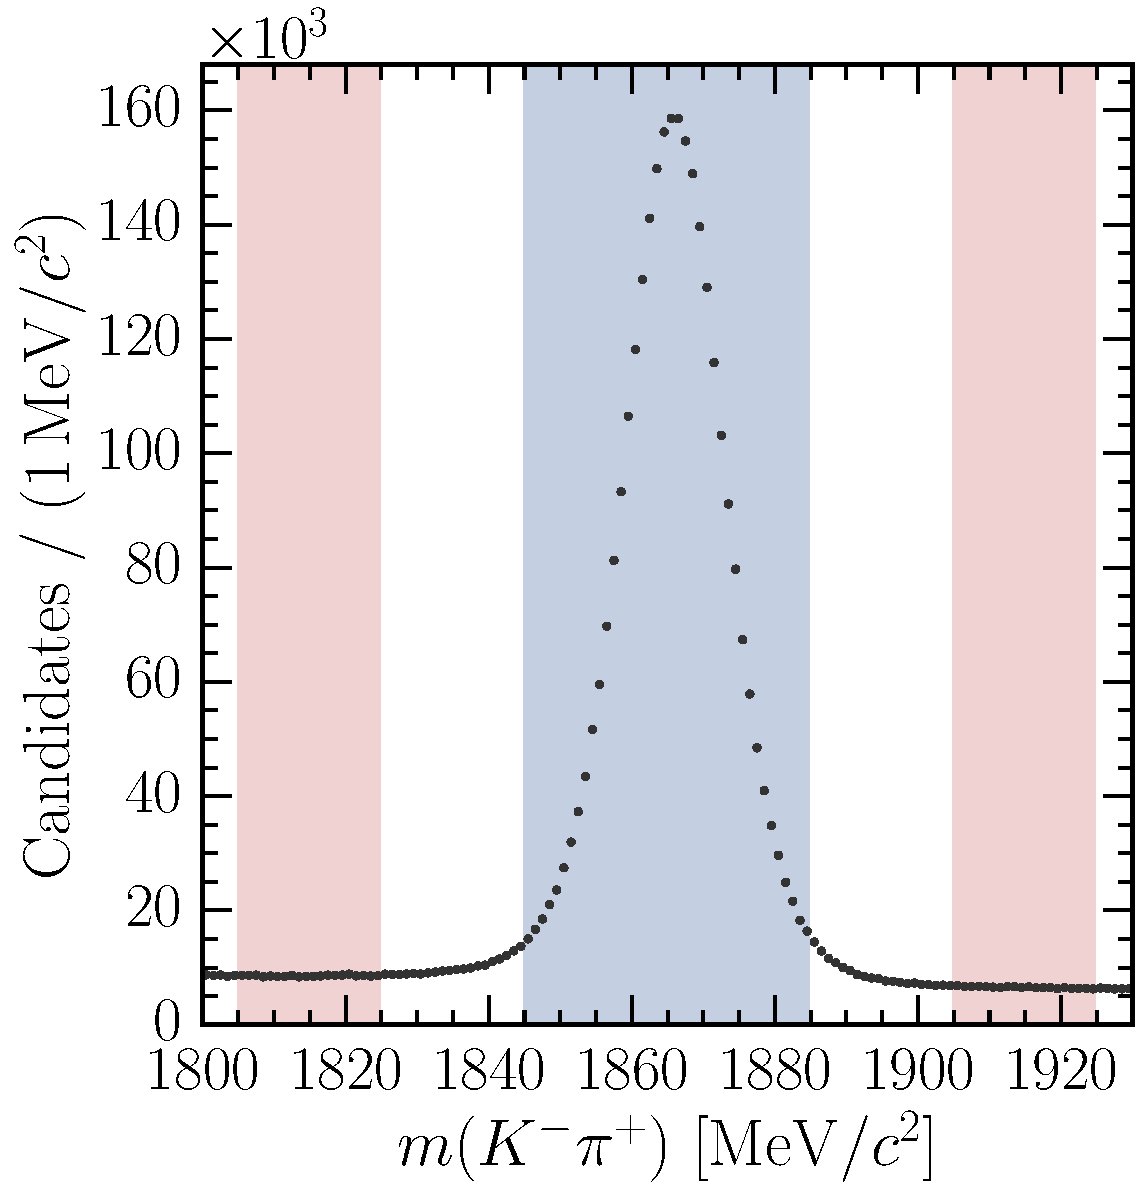
\includegraphics[width=\textwidth]{figures/production/fitting/D0ToKpi_mass_offline_selection_regions}
  \caption{%
    Definition of signal window, in blue, and sidebands, in red, for \DzToKpi\ 
    candidates.
    The signal window is $\pm\SI{20}{\MeV}$ either side of the nominal \PDzero 
    mass of \SI{1864.84}{\MeV}~\cite{PDG2014}.
    The upper and lower sidebands are each \SI{20}{\MeV} wide, with the lower 
    sideband ending \SI{40}{\MeV} below the nominal \PDzero mass and the upper 
    sideband beginning \SI{40}{\MeV} above the nominal \PDzero mass.
    The full dataset is shown.
  }
  \label{fig:prod:fitting:regions:D0ToKpi}
\end{figure}

\begin{figure}
  \centering
  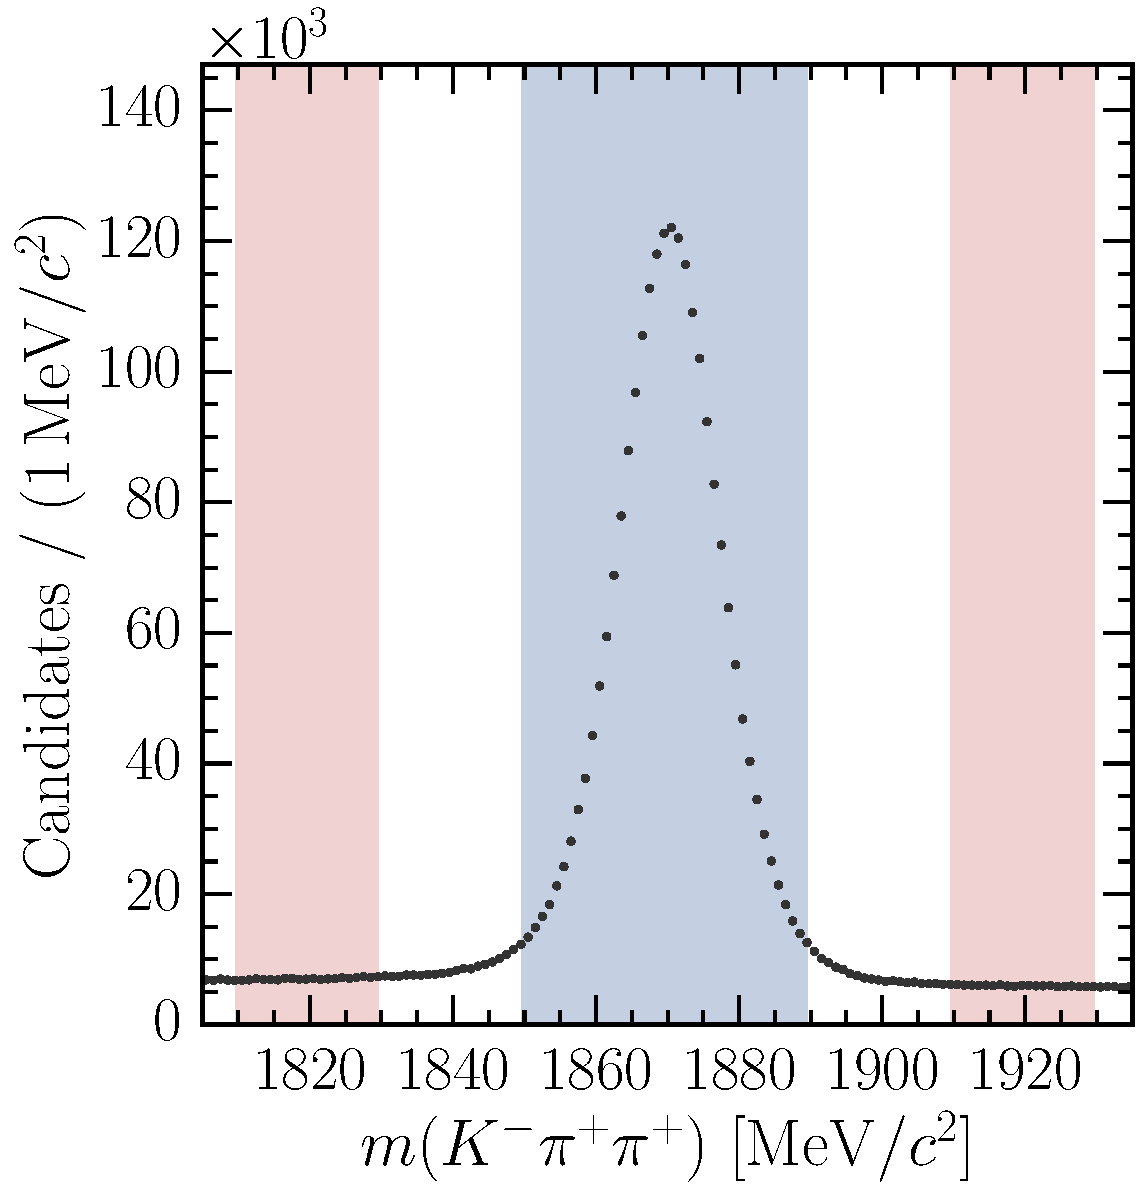
\includegraphics[width=\textwidth]{figures/production/fitting/DpToKpipi_mass_offline_selection_regions}
  \caption{%
    Definition of signal window, in blue, and sidebands, in red, for 
    \DpToKpipi\ candidates.
    The signal window is $\pm\SI{20}{\MeV}$ either side of the nominal \PDplus 
    mass of \SI{1869.61}{\MeV}~\cite{PDG2014}.
    The upper and lower sidebands are each \SI{20}{\MeV} wide, with the lower 
    sideband ending \SI{40}{\MeV} below the nominal \PDplus mass and the upper 
    sideband beginning \SI{40}{\MeV} above the nominal \PDplus mass.
    The full dataset is shown.
  }
  \label{fig:prod:fitting:regions:DpToKpipi}
\end{figure}

\begin{figure}
  \centering
  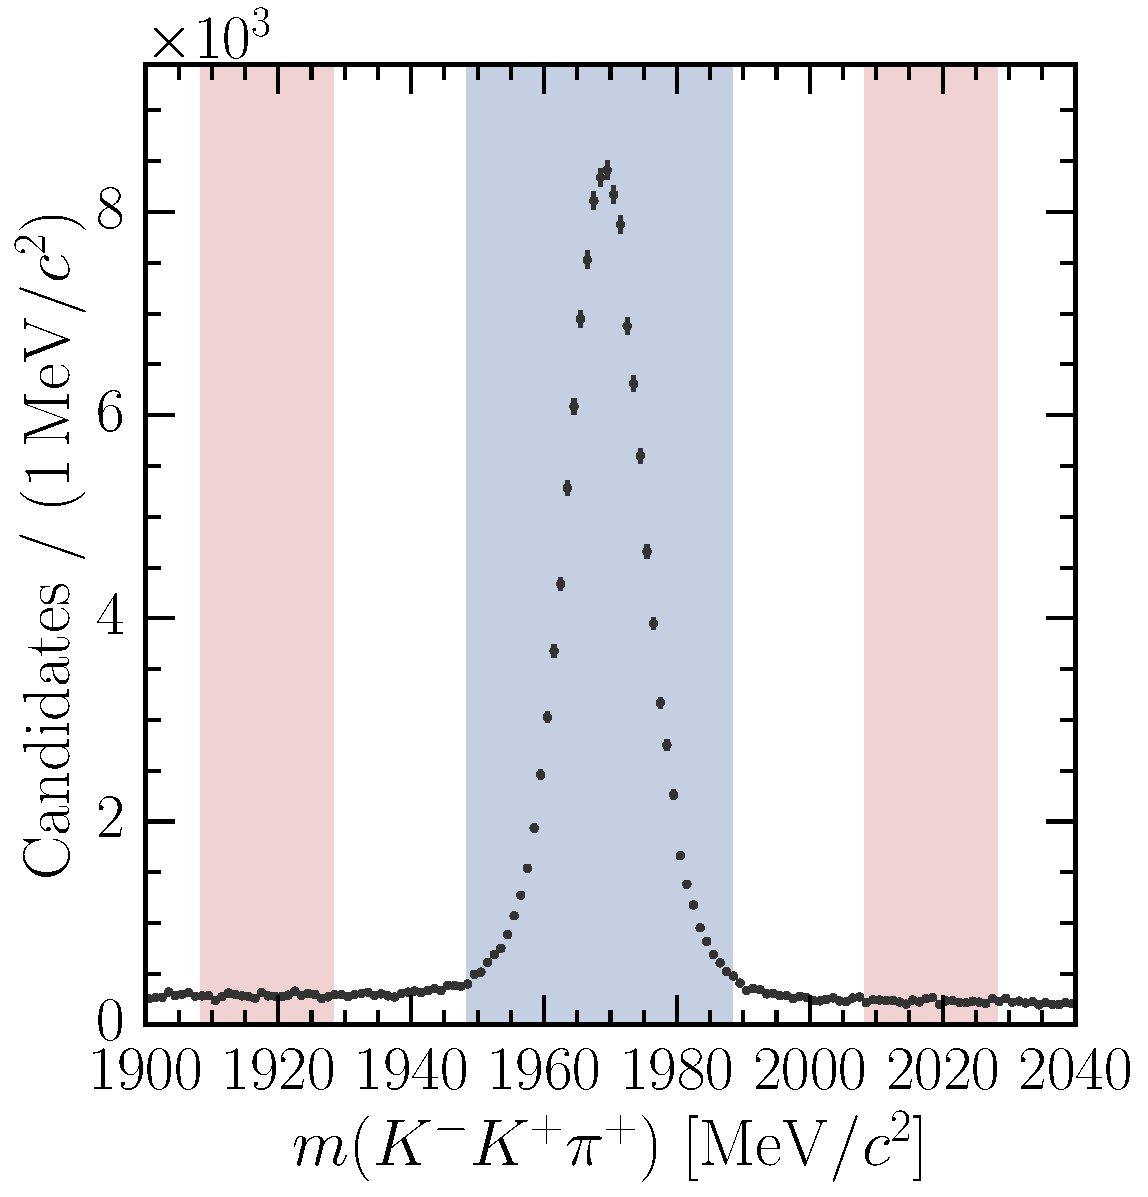
\includegraphics[width=\textwidth]{figures/production/fitting/DsToKKpi_mass_offline_selection_regions}
  \caption{%
    Definition of signal window, in blue, and sidebands, in red, for 
    \DspTophipi\ candidates.
    The signal window is $\pm\SI{20}{\MeV}$ either side of the nominal \PDsplus 
    mass of \SI{1968.30}{\MeV}~\cite{PDG2014}.
    The upper and lower sidebands are each \SI{20}{\MeV} wide, with the lower 
    sideband ending \SI{40}{\MeV} below the nominal \PDsplus mass and the upper 
    sideband beginning \SI{40}{\MeV} above the nominal \PDsplus mass.
    The full dataset is shown.
  }
  \label{fig:prod:fitting:regions:DsToKKpi}
\end{figure}

\begin{figure}
  \centering
  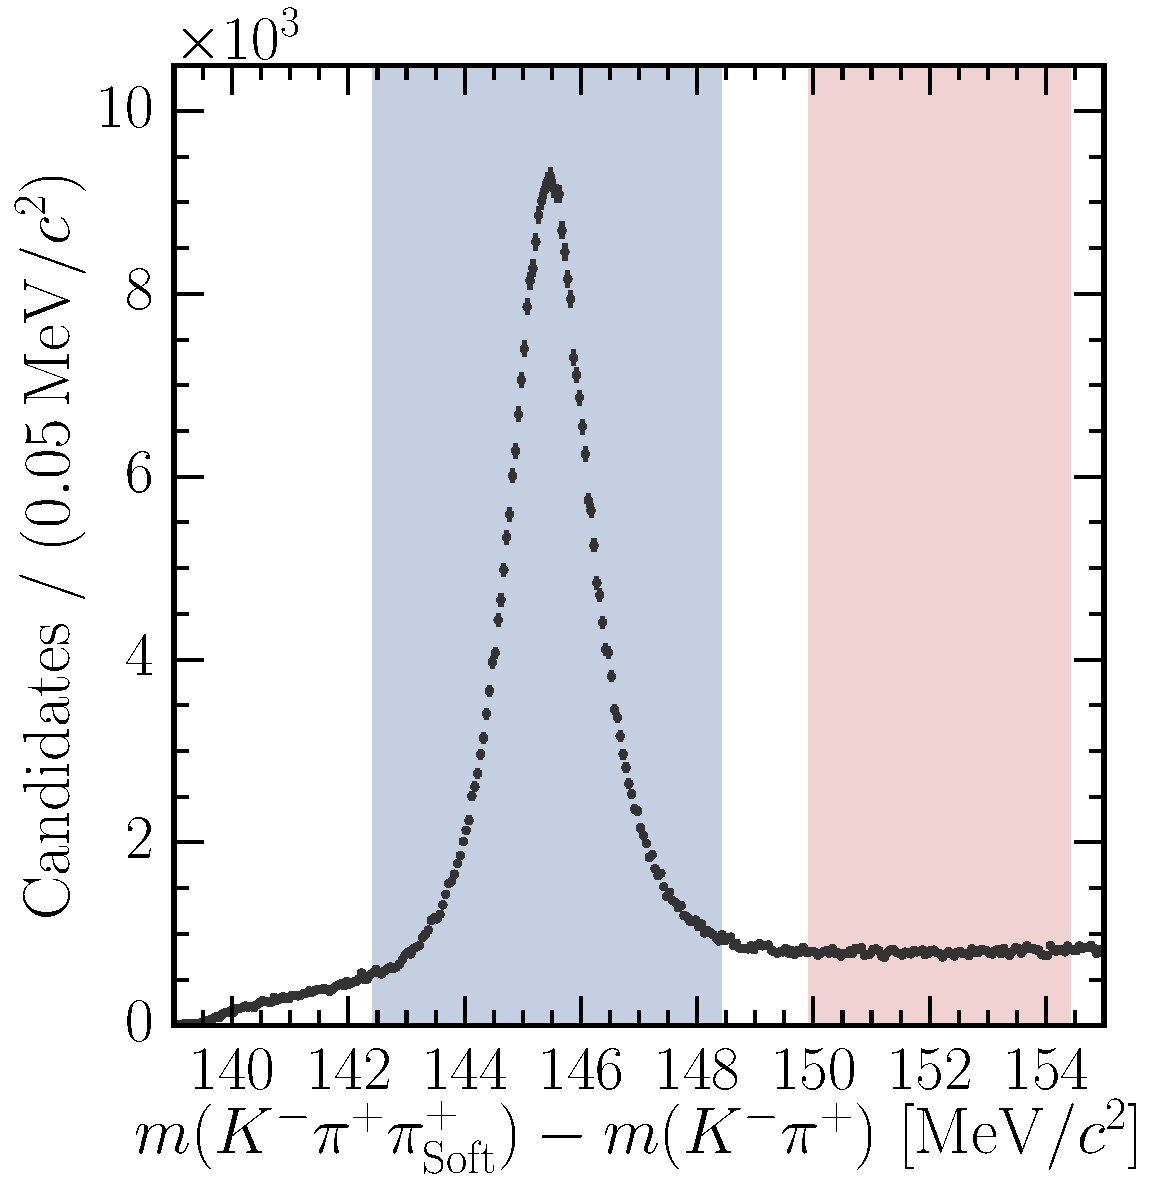
\includegraphics[width=\textwidth]{figures/production/fitting/DstToD0pi_D0ToKpi_delta_mass_offline_selection_regions}
  \caption{%
    Definition of signal window, in blue, and sidebands, in red, for 
    \DstToDzpi, with \DzToKpi, candidates.
    The signal window is $\pm\SI{3}{\MeV}$ either side of the nominal $\deltam 
    = m(\PDstarp) - m(\PDzero)$ mass of \SI{145.43}{\MeV}~\cite{PDG2014}.
    The upper sideband is \SI{4.5}{\MeV} wide, beginning \SI{4.5}{\MeV} above 
    the nominal \deltam\ value.
    The full dataset within the \PDzero signal region, given in 
    \cref{fig:prod:fitting:regions:D0ToKpi},is shown.
  }
  \label{fig:prod:fitting:regions:DstToD0pi_D0ToKpi}
\end{figure}

\section{Mass fits}
\label{chap:prod:fitting:mass}

For each one-dimensional mass and \deltam\ fit, one PDF is defined per 
discriminatory species: signal and combinatorial background.
In both the mass and \deltam\ distributions, the prompt and secondary signal 
shapes are assumed to be identical, and for the \deltam\ fits the combinatorial 
background is assumed to be indistinguishable from \emph{random soft pion} 
backgrounds, where a true \PDzero is combined with a random track in the event.
The total \ac{PDF} is constructed as the sum of the per-species \acp{PDF}, each $f_{s}$, 
each weighted by the respective yield $N_{s}$
\begin{align}
  f(m) &= \frac{1}{\sum_{\textnormal{s}} N_{\textnormal{s}}}
          \sum_{\textnormal{s}} N_{\textnormal{s}}
          f_{\textnormal{s}}(m),\\
  f(\deltam) &= \frac{1}{\sum_{\textnormal{s}} N_{\textnormal{s}}}
                \sum_{\textnormal{s}} N_{\textnormal{s}}
                f_{\textnormal{s}}(\deltam).
\end{align}

For every mass fit, the background PDF $f_{\textnormal{Bkg.}}(m)$ is taken to 
be a first-order polynomial, and the signal PDF $f_{\textnormal{Sig.}}(m)$ is 
dependent on the charm hadron candidate, given in 
Section~\ref{chap:prod:fitting:details}.

The combinatorial and random soft pion background in the \deltam\ fits is 
modelled as an empirical threshold function of the (un-normalised) form
\begin{equation}
  % (dm - dm0)^A * exp(B*dm)
  R(x; \deltam_{0}, A, B) = e^{B\deltam}
    {(x - \deltam_{0})}^A,
\end{equation}
where $\deltam_{0}$ is the threshold value, fixed to the charged pion rest mass 
$m_{\Ppipm} = \SI{139.57}{\MeV}$~\cite{PDG2014}, and the parameter $B$ is fixed 
to zero.
The signal PDF is the sum of three normal distributions, sharing a common mean 
but allowed to have varying widths.

One mass or \deltam\ PDF, $f(m)$ or $f(\deltam)$, is constructed per \pTy\ bin, 
and the likelihood is formed as the product of these such that each PDF is 
fitted simultaneously when the \ac{NLL} is minimised.

\section{\lnipchisq\ fit}
\label{chap:prod:fitting:ipchisq}

The prompt and secondary signal distributions are modelled by continuous, 
parametric \acp{PDF}.
Rather than attempting to parameterise the combinatorial background 
distribution, a \acf{KDE} \ac{PDF}, or `template', is created from the 
\lnipchisq\ distribution in the lower and upper sidebands of the reconstructed 
charm hadron mass.
In the case of the \PDstarp measurements, the upper sideband of the \deltam\ 
distribution is used instead.
This approach assumes that the \lnipchisq\ shape in the signal region is the 
same as that in the sidebands, that is that the mass and \lnipchisq\ are 
uncorrelated in the background sample.

The signal region in each long-lived charm hadron mass distribution is defined 
as a \SI{40}{\MeV}-wide window centred on the nominal rest mass of the given 
charm hadron, taken to be $m_{\PDzero} = \SI{1864.84}{\MeV}$, $m_{\PDplus} = 
\SI{1869.61}{MeV}$, and $m_{\PDsplus} = \SI{1968.30}{\MeV}$~\cite{PDG2014}.
The lower sideband is a \SI{20}{\MeV}-wide window centred \SI{50}{\MeV} below 
the centre of the signal window, and the upper sideband is a \SI{20}{\MeV}-wide 
window centred \SI{50}{\MeV} above the centre of the signal window.
For the \PDstarp\ measurements, the signal region is defined as a window 
\SI{6}{\MeV} wide, centred on the nominal \deltam\ value of 
\SI{145.43}{\MeV}~\cite{PDG2014}.
The upper sideband, or just `sideband' as a lower sideband region is not 
defined, is defined as the region from \SI{4.5}{\MeV} to \SI{9}{\MeV} above the 
centre of the signal region.
\Cref{fig:prod:fitting:regions:D0ToKpi,fig:prod:fitting:regions:DpToKpipi,fig:prod:fitting:regions:DsToKKpi,fig:prod:fitting:regions:DstToD0pi_D0ToKpi}
show the signal and sideband regions for each mode. A comparison between
the \lnipchisq\ distributions in the two sidebands is shown in 
Appendix~\ref{app:sidebands}.

The integral of the \lnipchisq\ background template \ac{PDF} is constrained to 
be near the number of background candidates in the signal region.
This number is measured with the binned maximum likelihood fit to the charm 
hadron mass distribution, or to the \deltam\ distribution in the \PDzero mass 
signal region for the \PDstarp\ measurements, as described in 
Section~\ref{chap:prod:fitting:mass}.
To avoid any complications due to correlations between the background template 
\ac{PDF} and the fitted data, only the data in signal region is used in the 
\lnipchisq\ fit.
For the \PDstarp\ measurements, this signal region requirement is made in both 
the \PDzero mass and the \deltam\ distributions.

For each one-dimensional \lnipchisq\ fit, we assign one \ac{PDF} $f_{s}$ per 
discriminatory species: prompt signal, secondary signal, and combinatorial 
background.
The total \acp{PDF} are constructed as the sum of per-species \acp{PDF}, 
each weighted by the respective yield $N_{s}$
\begin{equation}
  f(\lnipchisq) = \frac{1}{\sum_{\textnormal{s}} N_{\textnormal{s}}}
                  \sum_{\text{s}} N_{\text{s}}
                  f_{\text{s}}(\lnipchisq).
\end{equation}
The constraint on the background yield is applied by multiplying 
$f(\lnipchisq)$ by a normal distribution whose mean is the number of background 
candidates $N$ measured by the mass fit and whose width is the uncertainty on 
$N$ returned by the fitter.

One \lnipchisq\ \ac{PDF}, $f(\lnipchisq)$, and background constraint is 
constructed per \pTy\ bin, and the likelihood is formed as the product of these 
such that each \ac{PDF} is fitted simultaneously when the negative 
log-likelihood is minimised.
The benefit of this construction is that some shape parameters can be shared 
across bins, reducing the uncertainty on the fit parameters.
Which parameters are shared across bins and which are fitted independently is 
dependent on the final state, and are enumerated in 
\cref{chap:prod:fitting:details}.

The prompt signal model in the \lnipchisq\ distribution is a modified normal 
distribution $H$, where the width is allowed to be asymmetric with respect to 
the mean and the tails are described by exponential functions
\begin{equation}
  H(x; \mu, \sigma, \epsilon, \rho_{L}, \rho_{R}) =
  \begin{cases}
    \exp\left(\frac{\rho_{L}^{2}}{2} + \rho_{L}\frac{x - \mu}{(1 - 
    \epsilon)\sigma}\right) & x < \mu - (\rho_{L}\sigma(1 - 
        \epsilon)), \\
    \exp\left(-\left(\frac{x - \mu}{\sqrt{2}\sigma(1 - 
    \epsilon)}\right)^{2}\right) & \mu - (\rho_{L}\sigma(1 - \epsilon)) 
          \leq x < \mu, \\
    \exp\left(-\left(\frac{x - \mu}{\sqrt{2}\sigma(1 + 
    \epsilon)}\right)^{2}\right) & \mu \leq x < \mu + (\rho_{R}\sigma(1 + 
          \epsilon)), \\
    \exp\left(\frac{\rho_{R}^{2}}{2} - \rho_{R}\frac{x - \mu}{(1 + 
    \epsilon)\sigma}\right) & x \geq \mu + (\rho_{R}\sigma(1 + 
        \epsilon)),
  \end{cases}
\end{equation}
where the parameter $\mu$ is the mode of the distribution, $\sigma$ is the 
average of the left and right widths, $\epsilon$ is the asymmetry between the 
left and right widths, and $\rho_{L(R)}$ is the exponent for the left (right) 
tail.
The secondary signal distribution is modelled by a normal distribution $G$ with 
mean $\mu$ and width $\sigma$
\begin{equation}
  G(x; \mu, \sigma) = \frac{1}{\sqrt{2\pi}\sigma}
                      e^{-\frac{{(x - \mu)}^{2}}{2\sigma^{2}}}.
\end{equation}
These shapes are motivated by the \lnipchisq\ distributions for prompt and 
secondary signal decays observed in the \ac{MC} samples.

Given the large number of parameters to be fitted, some shape parameters are 
fixed to values obtained from `prefits' to samples of prompt and secondary 
signal \ac{MC}.
The set of parameters that are fixed is dependent on the charm meson, given in 
\cref{chap:prod:fitting:details}.

\section{Mode-specific details}
\label{chap:prod:fitting:details}

As different final states exhibit different features in the mass, \deltam, and 
\lnipchisq\ distributions, several aspects of the fits are different between 
modes.
This sections gives the list of parameters that are split between \pTy\ bins, 
and the list of parameters that are allowed to float after the fit to \ac{MC} 
data, for each mode.

Initially, no knowledge is assumed on which parameters should be independent 
(to be `split') across the \pTy\ bins, nor of whether the \lnipchisq\ 
distribution is well-modelled by the \ac{MC}.
The chosen parameterisation is that which best describes the data.
For the mass fits, all parameters are initially fixed such that they are same 
across all \pTy\ bins, and are then split one by one when it is observed that a 
feature varies across the bins, such as the width of the signal peak.
All parameters of the \lnipchisq\ fits are first kept fixed to values found 
from the fits to the simulated data, and then individual parameters are floated 
if the total PDF does not model the data well.
Parameters are then split across \pTy\ bins in the same manner as in the mass 
fits.

\subsection{Fit details for \PDzero}
\label{chap:prod:fitting:details:D0ToKpi}

For the \DzToKpi\ mode, the signal shape in the mass fit is the sum of a normal 
and a Crystal Ball distribution~\cite{Skwarnicki:1986xj}, sharing a common mean but allowed to have 
different widths.
The Crystal Ball function $C$ is a normal distribution but with a power-law 
tail on one side, defined (un-normalised) as
\begin{equation}
  C(x; \mu, \sigma, \alpha, n) = \begin{cases}
    e^{-\frac{{(x - \mu)}^{2}}{2\sigma^{2}}}                          & \frac{x - \mu}{\sigma} > -\alpha, \\
    e^{-\frac{|\alpha|^{2}}{2}}
      {(\frac{n}{|\alpha|})}^{n}
      {(\frac{n}{|\alpha|} - |\alpha| - \frac{x - \mu}{\sigma})}^{-n} & \frac{x - \mu}{\sigma} \leq -\alpha,
  \end{cases}
  \label{eqn:prod:fitting:crystal_ball}
\end{equation}
where $\alpha$ defines how far away from the mean $\mu$ the power-law tail 
begins, in units of the width of the core Gaussian $\sigma$, and $n$ is the 
power law exponent.
The mean and width of the total signal mass \ac{PDF} are split across \pTy\ 
bins, as is the slope of the background mass \ac{PDF}.
The mean of the \lnipchisq\ prompt signal \ac{PDF} and the width of the 
secondary signal \ac{PDF} are also split across \pTy\ bins.
The mean and width of the prompt signal \lnipchisq\ \ac{PDF} and all parameters 
of the secondary signal \lnipchisq\ \ac{PDF} are floated in the fit to data, 
and all other \lnipchisq\ shape parameters fixed to the values from \ac{MC}.

Prefits to the prompt signal and secondary signal data samples in \lnipchisq\ 
are given in \cref{fig:fitting:details:D0ToKpi-prefits}.

\subsubsection*{Fit details for \PDplus}
\label{chap:prod:fitting:details:D0ToKpi}

For the \DpToKpipi\ mode, the signal shape in the mass fit is the sum of a 
normal and a Crystal Ball distribution, sharing a common mean but allowed to 
have different widths.
The mean of the signal mass \ac{PDF} as well as the width of the Crystal Ball 
component in the mass \ac{PDF} are split across \pTy\ bins, as is the slope of 
the background mass \ac{PDF}.
The mean of the \lnipchisq\ prompt signal and secondary signal distributions 
are split across \pTy\ bins.
The mean and tail parameters of the signal \lnipchisq\ \ac{PDF}, are floated 
during the fit to data, with all other shape parameters fixed to the values 
from \ac{MC}.

Prefits to the prompt signal and secondary signal data samples in \lnipchisq\ 
are given in \cref{fig:fitting:details:DpToKpipi-prefits}.

\subsubsection*{Fit details for \PDsplus}
\label{chap:prod:fitting:details:DsToKKpi}

For the \DspTophipi\ mode, the signal shape in the mass fit is the sum of a two 
normal distributions, sharing a common mean but allowed to have different 
widths.
The mean and width of the signal mass \ac{PDF} and the slope of the background 
mass \ac{PDF}, along with the mean of the \lnipchisq\ prompt signal \ac{PDF}, 
are split across \pTy\ bins.
The mean of the prompt signal \lnipchisq\ \ac{PDF} and all parameters of the 
secondary \ac{PDF} are floated during the fit to data, with all other shape 
parameters fixed to the values from \ac{MC}.

Prefits to the prompt signal and secondary signal data samples in \lnipchisq\ 
are given in \cref{fig:fitting:details:DsTophipi-prefits}.

\subsubsection*{Fit details for \PDstarp}
\label{chap:prod:fitting:details:DstToD0pi}

For the \PDstarp-tagged \DzToKpi\ mode, the width of the widest component of 
the signal model, described in \cref{chap:prod:fitting:mass}, is split across 
\pTy\ bins, along with the mean of the prompt signal \lnipchisq\ \ac{PDF}.
The mean of the prompt signal \lnipchisq\ \ac{PDF} and all parameters of the 
secondary \ac{PDF} are floated during the fit to data, with all other shape 
parameters fixed to the values from \ac{MC}.

Prefits to the prompt signal and secondary signal data samples in \PDzero 
\lnipchisq\ are given in \cref{fig:fitting:details:DstToD0pi_D0ToKpi-prefits}.

\subsection{Fit results}
\label{chap:prod:fitting:results}

For all fits, the covariance matrix is checked to be positive definite, and the 
goodness-of-fit within each \pTy\ bin is checked visually to ensure that the 
\ac{NLL} minimisation converged to a parameter set.
Mass, \deltam, and \lnipchisq\ fits are given in 
\cref{fig:prod:fitting:D0ToKpi,fig:prod:fitting:DpToKpipi,fig:prod:fitting:DsToKKpi,fig:prod:fitting:DstToD0pi_D0ToKpi}, 
where the data and models shown are the sums of the data and models from the 
\pTy\ bins.
Prompt signal yields per \pTy\ bin are given in 
\cref{tab:prod:fitting:D0ToKpi,tab:prod:fitting:DpToKpipi,tab:prod:fitting:DsToKKpi,tab:prod:fitting:DstToD0pi_D0ToKpi}, 
and those integrated across all bins in \cref{tab:prod:fitting:integrated}.

The plots show that the models match the data well, but there are some 
significant discrepancies such as in 
\cref{fig:prod:fitting:DsToKKpi:ipchisq,fig:prod:fitting:DstToD0pi_D0ToKpi:delta_mass}.
However, the discrepancies in these integrated plots are exaggerations of those 
in the individual \pTy\ bin fits: they indicate that there is a consistent bias 
in the individual bins, but do not necessarily indicate that these are 
statistically significant.
For comparison, 
\cref{fig:prod:fitting:D0ToKpi:sig_bkg,fig:prod:fitting:DpToKpipi:sig_bkg,fig:prod:fitting:DsToKKpi:sig_bkg,fig:prod:fitting:DstToD0pi_D0ToKpi:sig_bkg} 
show the mass (or \deltam) and \lnipchisq\ fits in the \pTy\ bin with the 
highest prompt signal yield and in the \pTy\ bin with the highest combinatorial 
background yield.
These show that, in the individual \pTy\ bins, the fits model the data 
significantly better than the integrated plots would suggest, and also that the 
fit is flexible enough to model both high prompt signal and high combinatorial 
background datasets.
The effect of the cross-section measurements of mis-modelling will be discussed 
further in \cref{chap:prod:systs}.

In some \pTy\ bins, it is not possible to make a prompt signal yield 
measurement due to insufficient data in those bins.
At this stage in the analysis, a cross-section measurement in a bin is 
considered infeasible if there is either no data (zero candidates), or if the 
prompt signal yield $N_{i} \pm \sigma_{N_{i}}$ in that bin as determined in the 
fit does not satisfy $N_{i} > 3\sigma_{N_{i}}$.

\begin{figure}
  \begin{subfigure}[b]{0.5\textwidth}
    \centering
    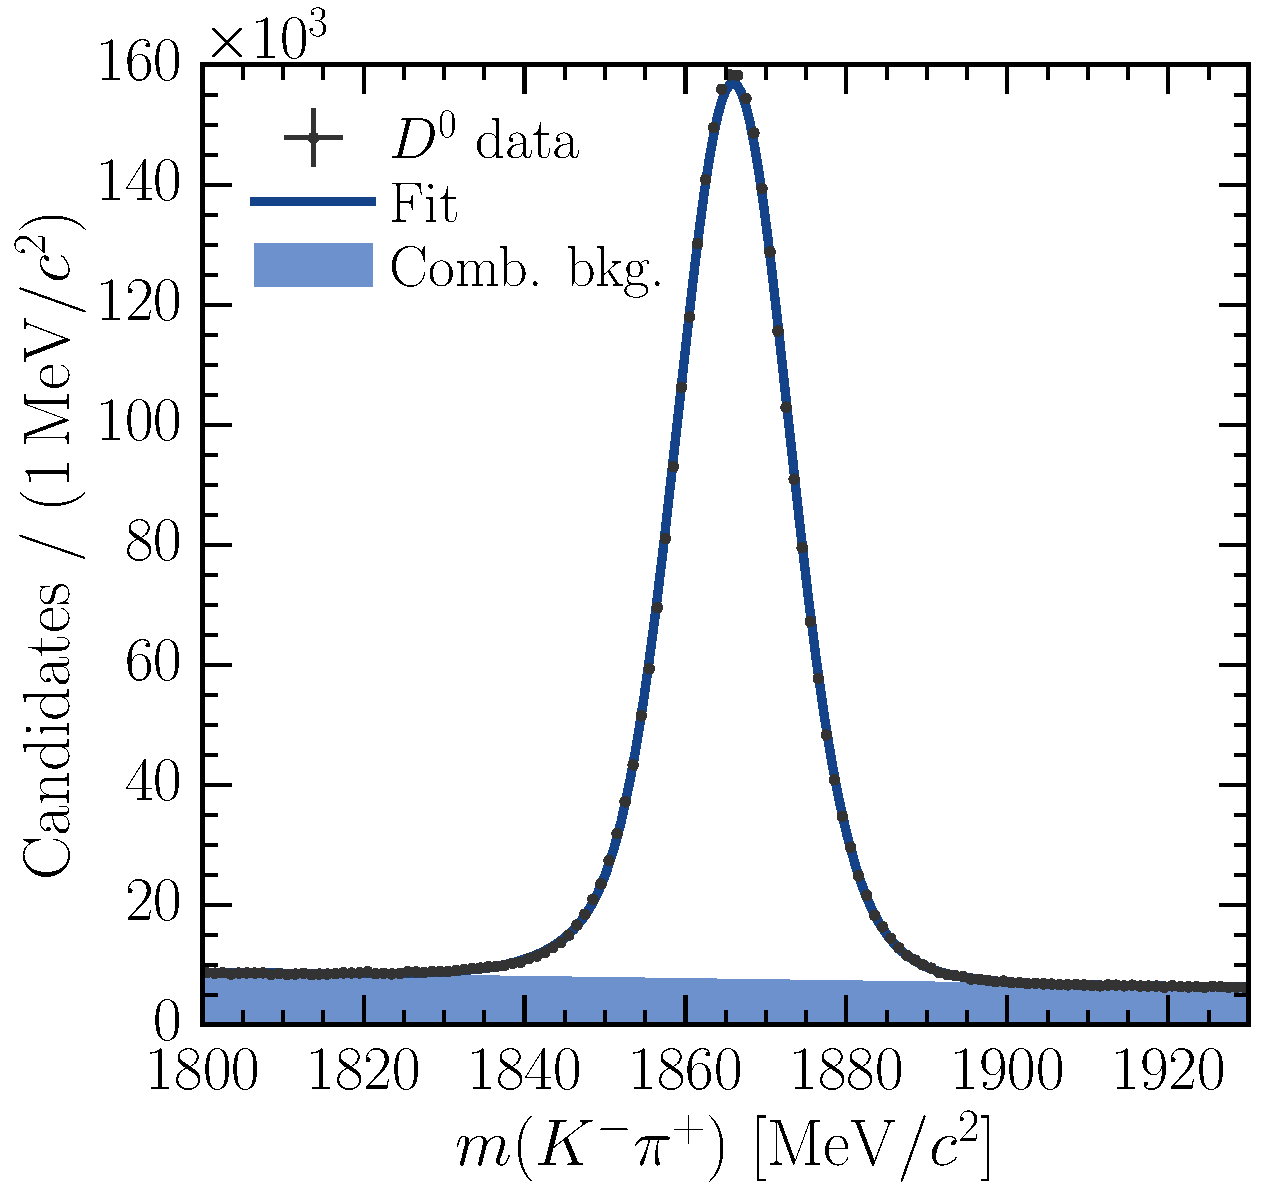
\includegraphics[width=\textwidth]{figures/production/fitting/D0ToKpi_mass_fit_pT_integrated_y_integrated}
    \caption{Mass}
    \label{fig:prod:fitting:D0ToKpi:mass}
  \end{subfigure}
  \begin{subfigure}[b]{0.5\textwidth}
    \centering
    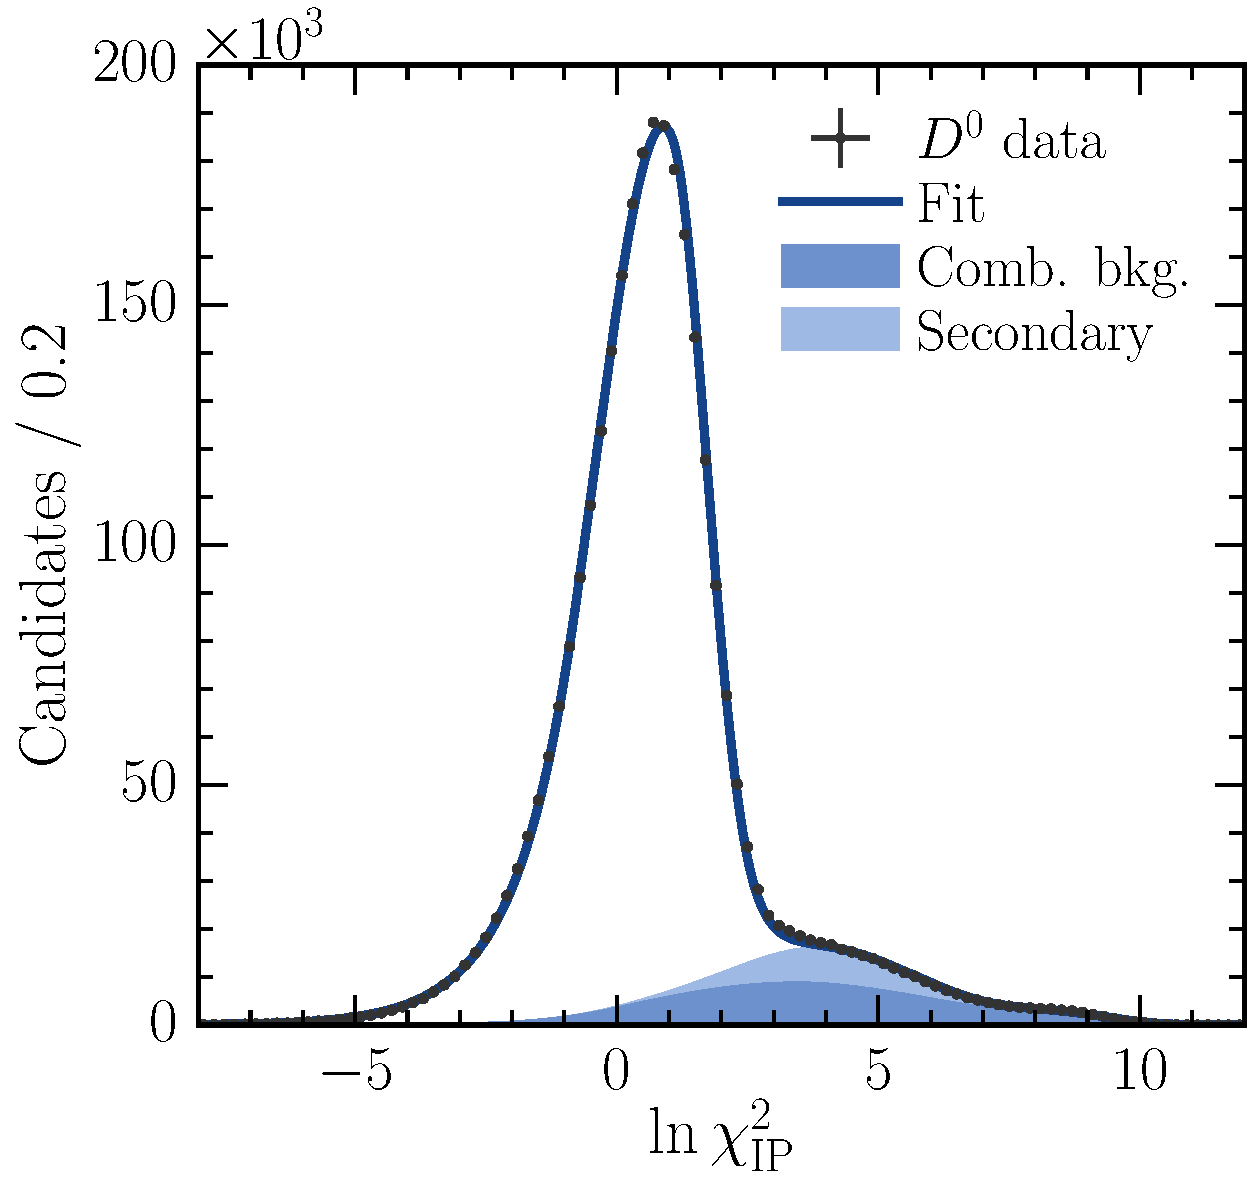
\includegraphics[width=\textwidth]{figures/production/fitting/D0ToKpi_ipchisq_fit_pT_integrated_y_integrated}
    \caption{\lnipchisq}
    \label{fig:prod:fitting:D0ToKpi:ipchisq}
  \end{subfigure}
  \caption{%
    Distributions for fully selected \DzToKpi\ candidates: \PDzero\ invariant 
    mass (\subref*{fig:prod:fitting:D0ToKpi:mass}); and \PDzero\ \lnipchisq\ 
    (\subref*{fig:prod:fitting:D0ToKpi:ipchisq}) for a mass window of 
    $\pm\SI{20}{\MeV}$ around the nominal \PDzero mass.
    The sum of the simultaneous likelihood fits in each \pTy\ bin is shown, 
    with components as indicated in the legends.
  }
  \label{fig:prod:fitting:D0ToKpi}
\end{figure}

\begin{figure}
  \begin{subfigure}[b]{0.5\textwidth}
    \centering
    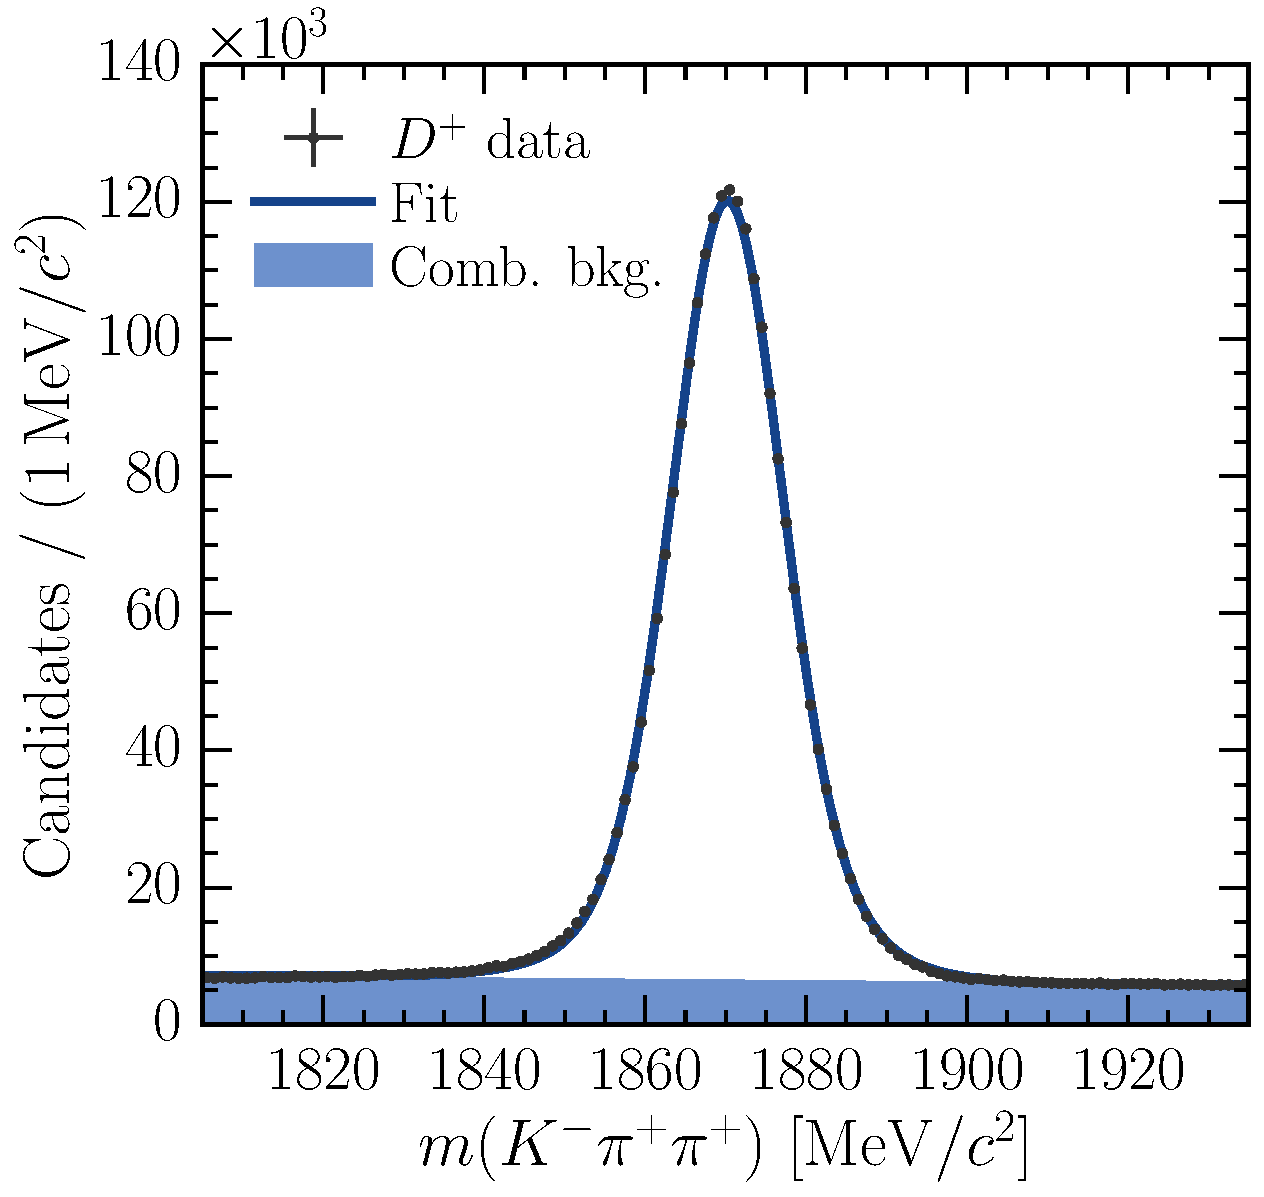
\includegraphics[width=\textwidth]{figures/production/fitting/DpToKpipi_mass_fit_pT_integrated_y_integrated}
    \caption{Mass}
    \label{fig:prod:fitting:DpToKpipi:mass}
  \end{subfigure}
  \begin{subfigure}[b]{0.5\textwidth}
    \centering
    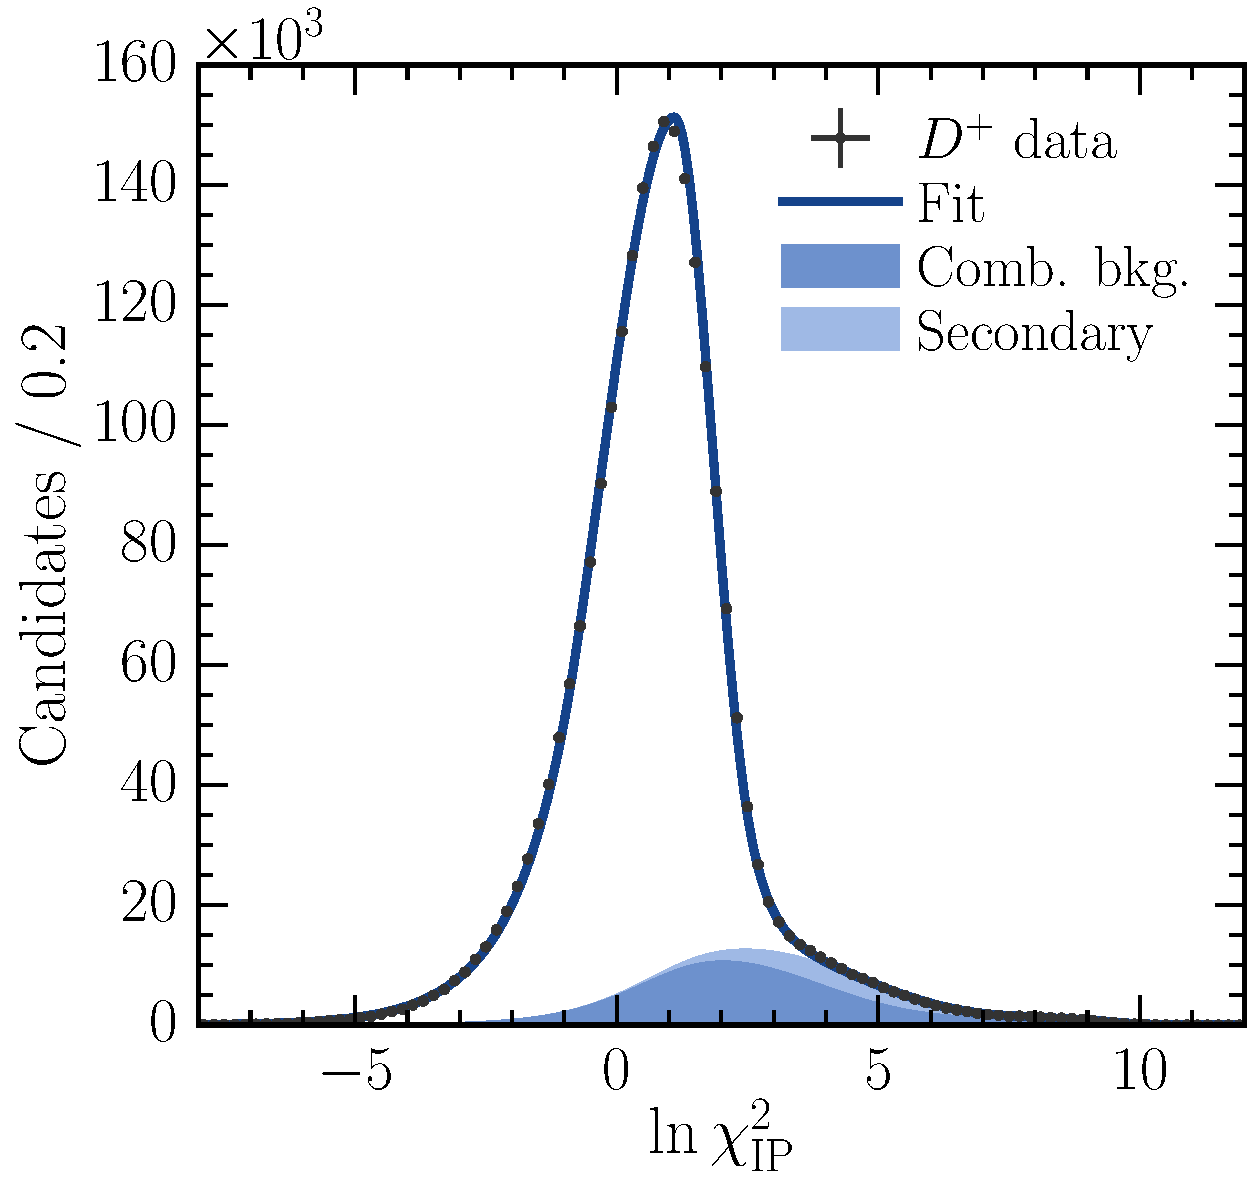
\includegraphics[width=\textwidth]{figures/production/fitting/DpToKpipi_ipchisq_fit_pT_integrated_y_integrated}
    \caption{\lnipchisq}
    \label{fig:prod:fitting:DpToKpipi:ipchisq}
  \end{subfigure}
  \caption{%
    Distributions for fully selected \DpToKpipi\ candidates: \PDplus\ invariant 
    mass (\subref*{fig:prod:fitting:DpToKpipi:mass}); and \PDplus\ \lnipchisq\ 
    (\subref*{fig:prod:fitting:DpToKpipi:ipchisq}) for a mass window of 
    $\pm\SI{20}{\MeV}$ around the nominal \PDplus mass.
    The sum of the simultaneous likelihood fits in each \pTy\ bin is shown, 
    with components as indicated in the legends.
  }
  \label{fig:prod:fitting:DpToKpipi}
\end{figure}

\begin{figure}
  \begin{subfigure}[b]{0.5\textwidth}
    \centering
    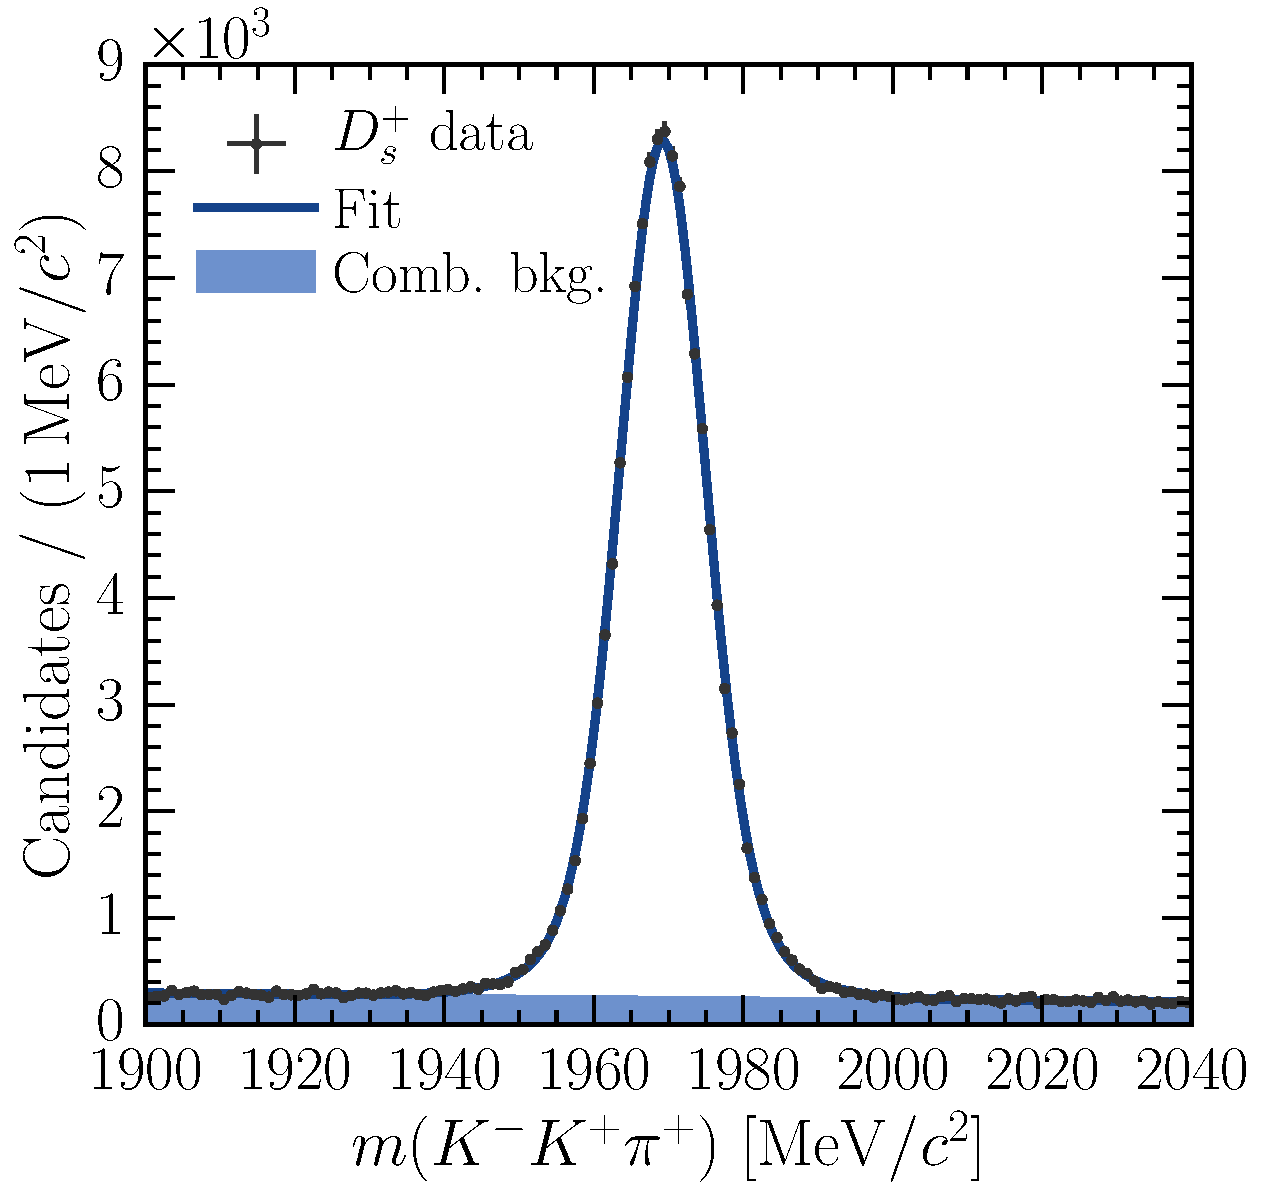
\includegraphics[width=\textwidth]{figures/production/fitting/DsToKKpi_mass_fit_pT_integrated_y_integrated}
    \caption{Mass}
    \label{fig:prod:fitting:DsToKKpi:mass}
  \end{subfigure}
  \begin{subfigure}[b]{0.5\textwidth}
    \centering
    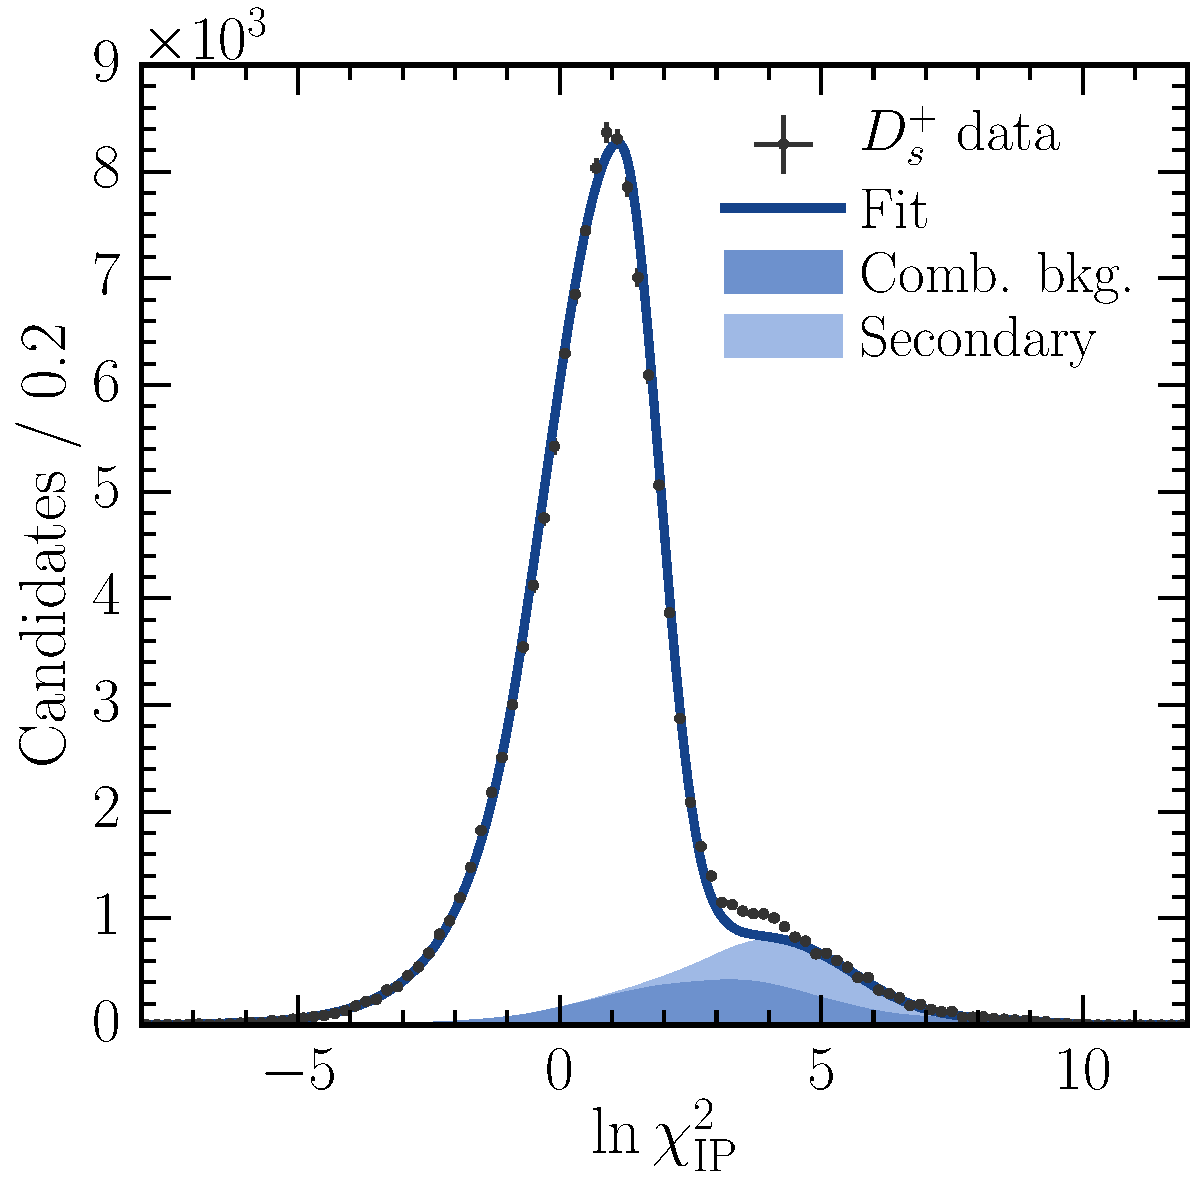
\includegraphics[width=\textwidth]{figures/production/fitting/DsToKKpi_ipchisq_fit_pT_integrated_y_integrated}
    \caption{\lnipchisq}
    \label{fig:prod:fitting:DsToKKpi:ipchisq}
  \end{subfigure}
  \caption{%
    Distributions for fully selected \DspTophipi\ candidates: \PDsplus\ 
    invariant mass (\subref*{fig:prod:fitting:DpToKpipi:mass}); and \PDsplus\ 
    \lnipchisq\ (\subref*{fig:prod:fitting:DpToKpipi:ipchisq}) for a mass 
    window of $\pm\SI{20}{\MeV}$ around the nominal \PDsplus mass.
    The sum of the simultaneous likelihood fits in each \pTy\ bin is shown, 
    with components as indicated in the legends.
  }
  \label{fig:prod:fitting:DsToKKpi}
\end{figure}

\begin{figure}
  \begin{subfigure}[b]{0.5\textwidth}
    \centering
    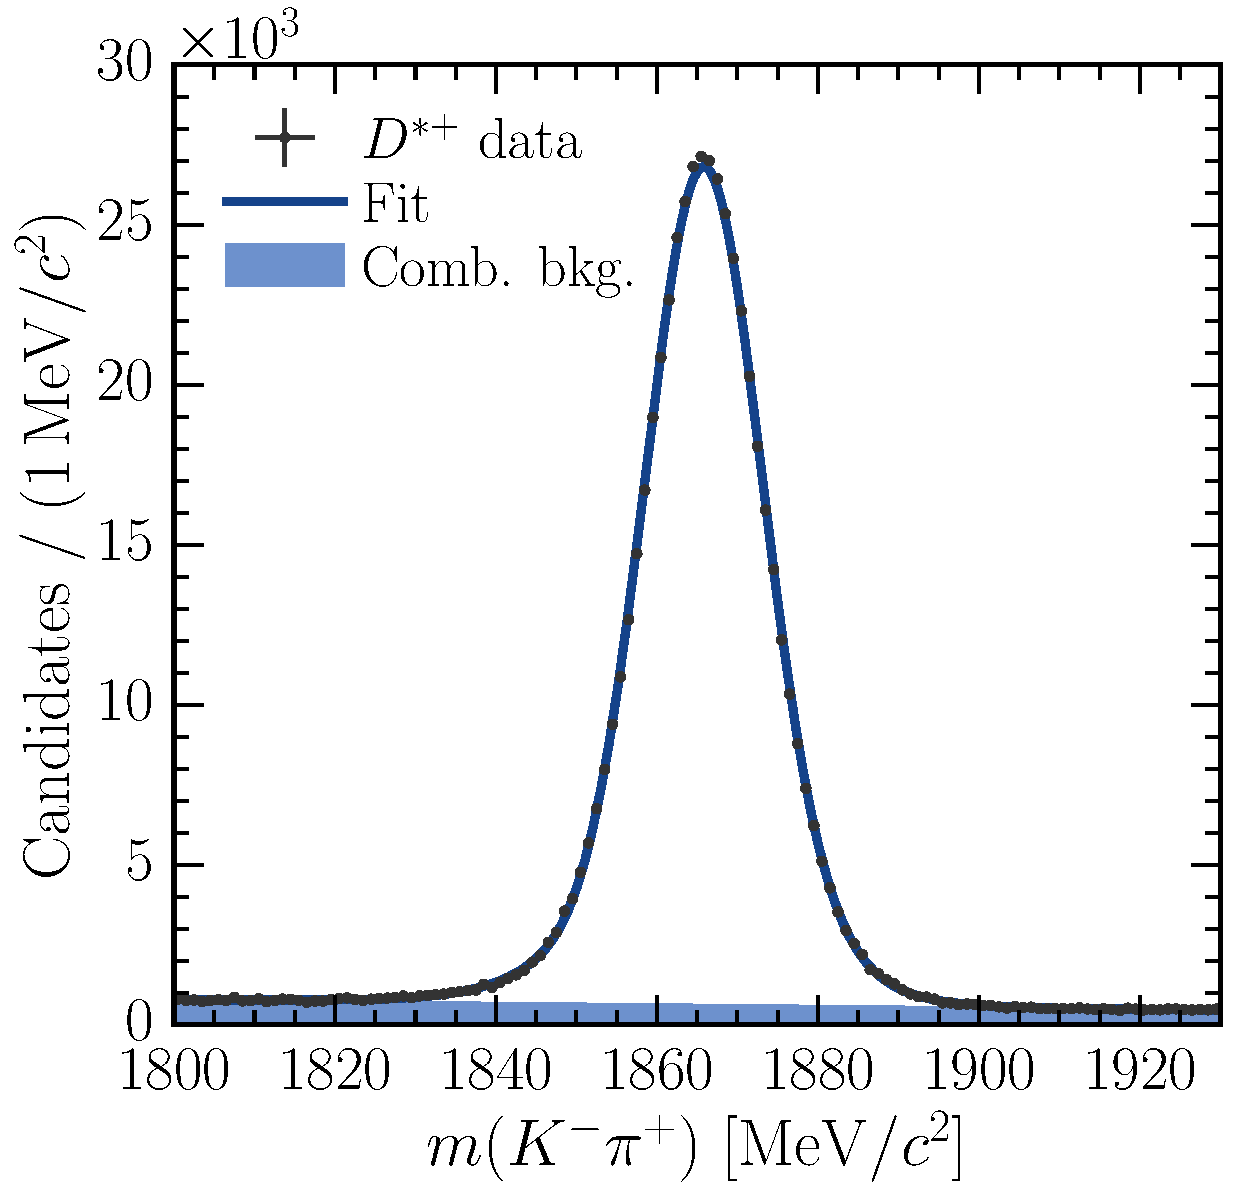
\includegraphics[width=\textwidth]{figures/production/fitting/DstToD0pi_D0ToKpi_mass_fit_pT_integrated_y_integrated}
    \caption{\PDzero mass}
    \label{fig:prod:fitting:DstToD0pi_D0ToKpi:mass}
  \end{subfigure}
  \begin{subfigure}[b]{0.5\textwidth}
    \centering
    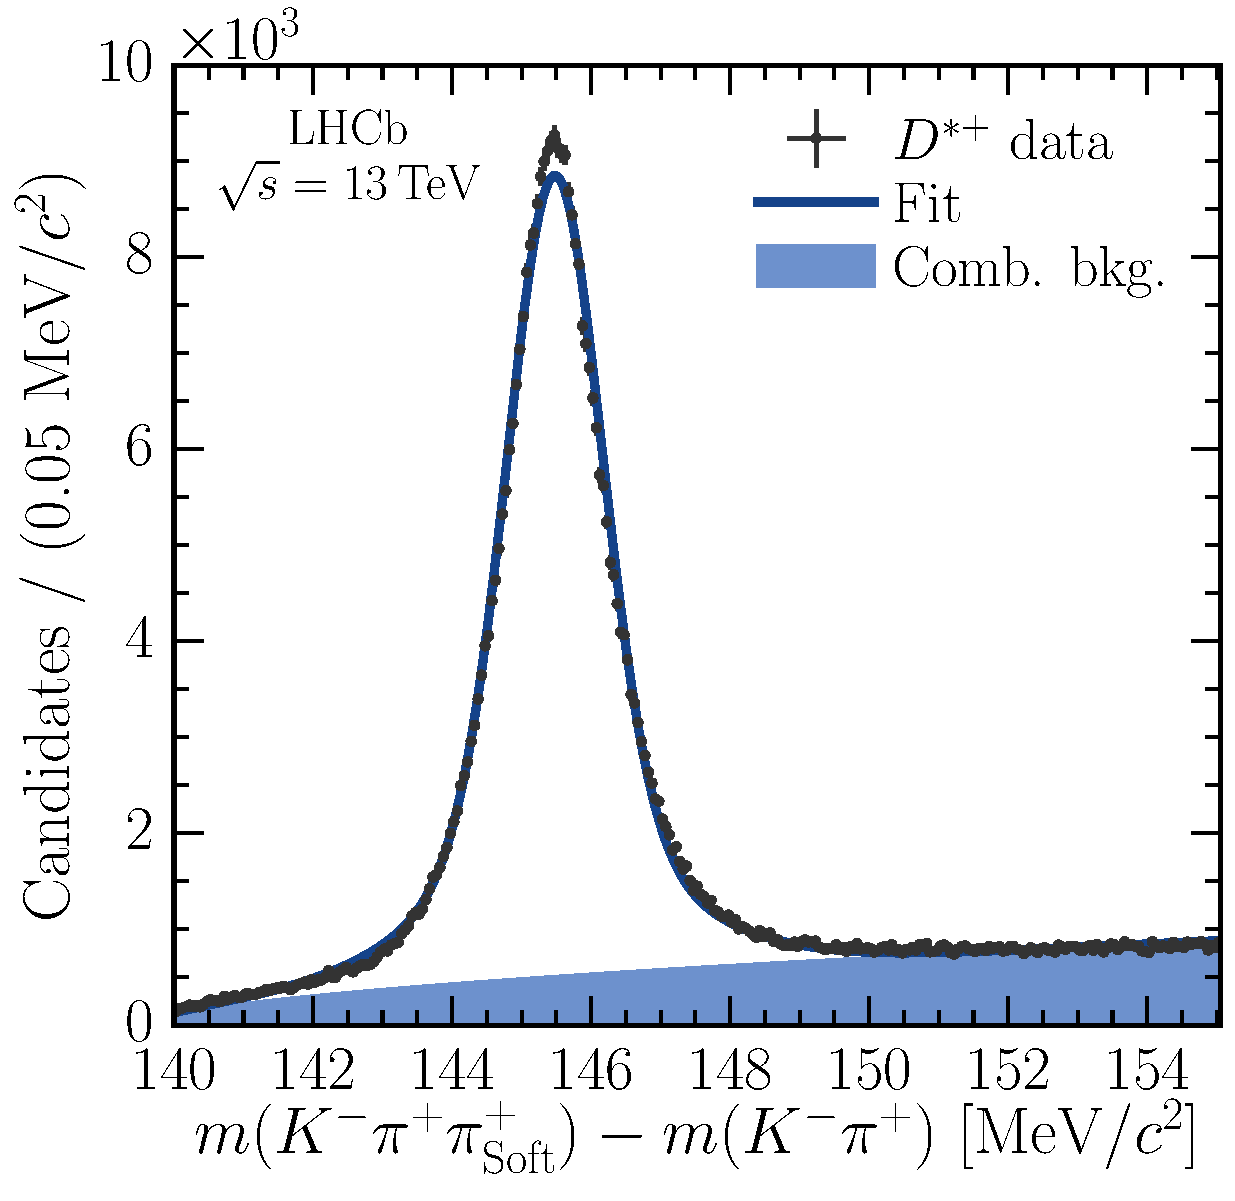
\includegraphics[width=\textwidth]{figures/production/fitting/DstToD0pi_D0ToKpi_delta_mass_fit_pT_integrated_y_integrated}
    \caption{Delta mass}
    \label{fig:prod:fitting:DstToD0pi_D0ToKpi:delta_mass}
  \end{subfigure}
  \begin{subfigure}[b]{0.5\textwidth}
    \centering
    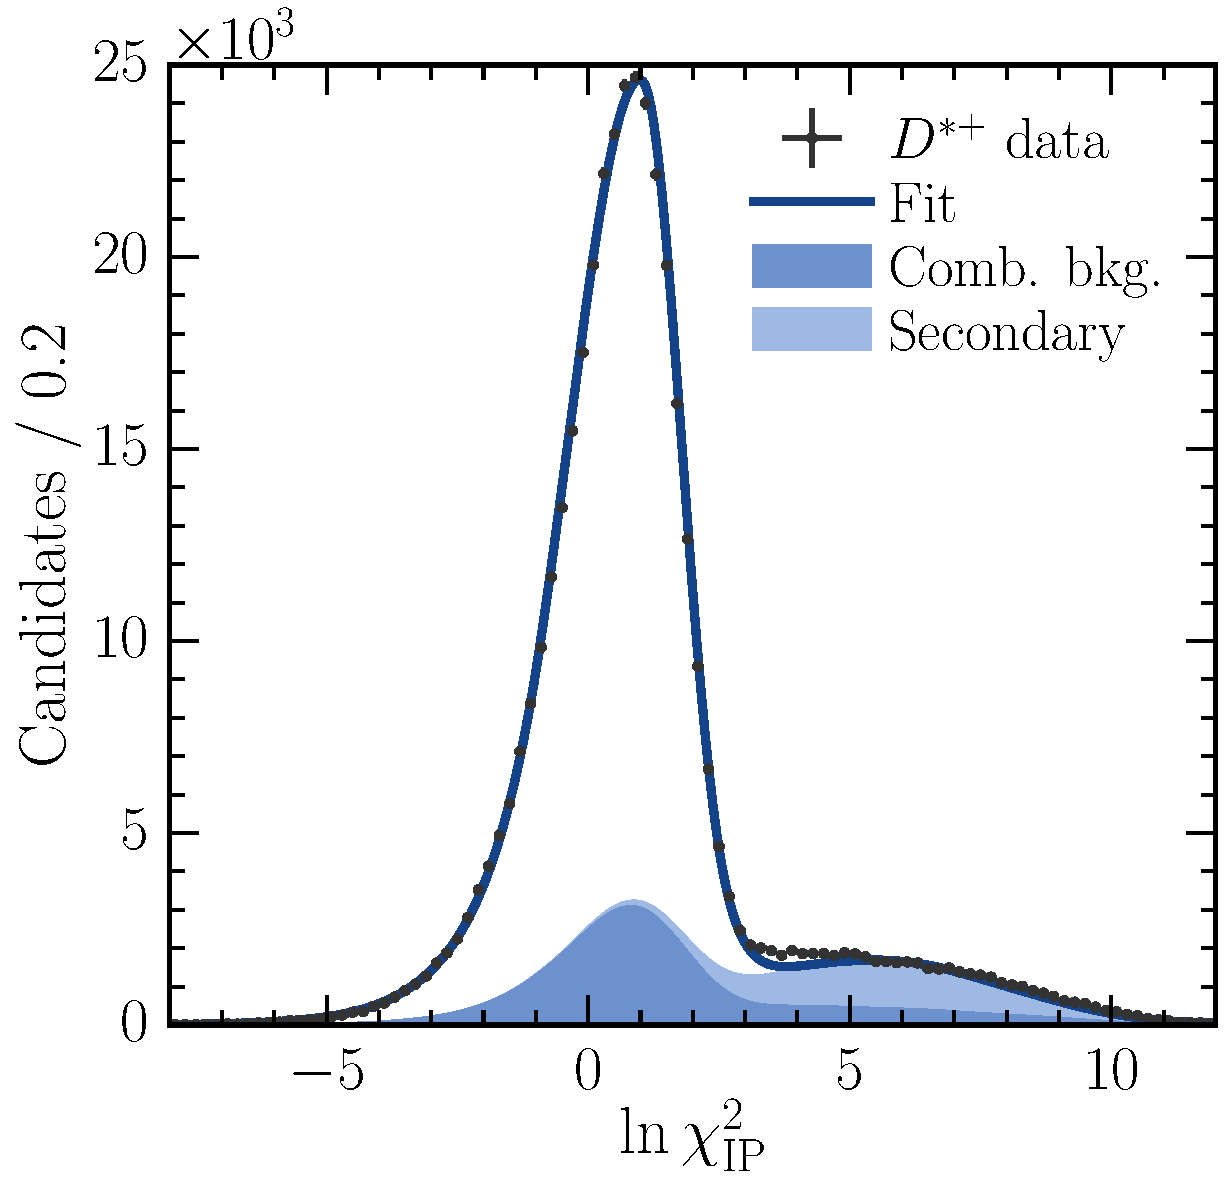
\includegraphics[width=\textwidth]{figures/production/fitting/DstToD0pi_D0ToKpi_ipchisq_fit_pT_integrated_y_integrated}
    \caption{\lnipchisq}
    \label{fig:prod:fitting:DstToD0pi_D0ToKpi:ipchisq}
  \end{subfigure}
  \caption{%
    Distributions for fully selected \PDstarp\ candidates, with \DzToKpi: 
    \PDzero\ invariant mass 
    (\subref*{fig:prod:fitting:DstToD0pi_D0ToKpi:mass}); $\deltam = m(\PDstarp) 
    - m(\PDzero)$ (\subref*{fig:prod:fitting:DstToD0pi_D0ToKpi:delta_mass}) for 
    a mass window of $\pm\SI{20}{\MeV}$ around the nominal \PDzero mass; and 
    \PDzero\ \lnipchisq\ (\subref*{fig:prod:fitting:DstToD0pi_D0ToKpi:ipchisq}) 
    with an additional mass window of $\pm\SI{3}{\MeV}$ around the nominal 
    \PDstarp-\PDzero\ mass difference.
    The sum of the simultaneous likelihood fits in each \pTy\ bin is shown, 
    with components as indicated in the legends.
  }
  \label{fig:prod:fitting:DstToD0pi_D0ToKpi}
\end{figure}

% TODO proper rounding in these tables
\begin{table}
  \caption{%
    Prompt signal yields for \DzToKpi\ measured in \PDzero \pTy\ bins.
    Cells marked with a dash `-' indicate bins where insufficient data were 
    available for a statistically significant prompt signal yield measurement.
  }
  \label{tab:prod:fitting:D0ToKpi}
  \centering
  \renewcommand{\arraystretch}{1.0}
\begin{tabular}{lr@{\hskip+0.2em}c@{\hskip+0.2em}r@{\hskip+0.2em}c@{\hskip+0.2em}rr@{\hskip+0.2em}c@{\hskip+0.2em}r@{\hskip+0.2em}c@{\hskip+0.2em}rr@{\hskip+0.2em}c@{\hskip+0.2em}r@{\hskip+0.2em}c@{\hskip+0.2em}rr@{\hskip+0.2em}c@{\hskip+0.2em}r@{\hskip+0.2em}c@{\hskip+0.2em}rr@{\hskip+0.2em}c@{\hskip+0.2em}r@{\hskip+0.2em}c@{\hskip+0.2em}r}
\toprule&\multicolumn{25}{c}{$y$}\\
$p_{\text{T}} [\text{MeV}/c]$ & \multicolumn{5}{c}{$[2,2.5]$} & \multicolumn{5}{c}{$[2.5,3]$} & \multicolumn{5}{c}{$[3,3.5]$} & \multicolumn{5}{c}{$[3.5,4]$} & \multicolumn{5}{c}{$[4,4.5]$} \\
\midrule$[14000,15000]$ & \multicolumn{5}{c}{$550 \pm 30$} & \multicolumn{5}{c}{$610 \pm 30$} & \multicolumn{5}{c}{$72 \pm 9$} & \multicolumn{5}{c}{ } & \multicolumn{5}{c}{ } \\
$[13000,14000]$ & \multicolumn{5}{c}{$860 \pm 30$} & \multicolumn{5}{c}{$970 \pm 40$} & \multicolumn{5}{c}{$180 \pm 20$} & \multicolumn{5}{c}{ } & \multicolumn{5}{c}{ } \\
$[12000,13000]$ & \multicolumn{5}{c}{$1250 \pm 40$} & \multicolumn{5}{c}{$1580 \pm 40$} & \multicolumn{5}{c}{$420 \pm 30$} & \multicolumn{5}{c}{ } & \multicolumn{5}{c}{ } \\
$[11000,12000]$ & \multicolumn{5}{c}{$1910 \pm 50$} & \multicolumn{5}{c}{$2520 \pm 50$} & \multicolumn{5}{c}{$890 \pm 30$} & \multicolumn{5}{c}{ } & \multicolumn{5}{c}{ } \\
$[10000,11000]$ & \multicolumn{5}{c}{$2990 \pm 60$} & \multicolumn{5}{c}{$3890 \pm 70$} & \multicolumn{5}{c}{$1880 \pm 50$} & \multicolumn{5}{c}{$32 \pm 6$} & \multicolumn{5}{c}{ } \\
$[9000,10000]$ & \multicolumn{5}{c}{$4830 \pm 70$} & \multicolumn{5}{c}{$6420 \pm 80$} & \multicolumn{5}{c}{$3810 \pm 70$} & \multicolumn{5}{c}{$170 \pm 20$} & \multicolumn{5}{c}{ } \\
$[8000,9000]$ & \multicolumn{5}{c}{$7570 \pm 90$} & \multicolumn{5}{c}{$10900 \pm 200$} & \multicolumn{5}{c}{$7250 \pm 90$} & \multicolumn{5}{c}{$680 \pm 30$} & \multicolumn{5}{c}{ } \\
$[7000,8000]$ & \multicolumn{5}{c}{$12000 \pm 200$} & \multicolumn{5}{c}{$18600 \pm 200$} & \multicolumn{5}{c}{$13700 \pm 200$} & \multicolumn{5}{c}{$2460 \pm 50$} & \multicolumn{5}{c}{ } \\
$[6000,7000]$ & \multicolumn{5}{c}{$19100 \pm 200$} & \multicolumn{5}{c}{$32400 \pm 200$} & \multicolumn{5}{c}{$25500 \pm 200$} & \multicolumn{5}{c}{$7510 \pm 90$} & \multicolumn{5}{c}{$39 \pm 6$} \\
$[5000,6000]$ & \multicolumn{5}{c}{$30100 \pm 200$} & \multicolumn{5}{c}{$56300 \pm 300$} & \multicolumn{5}{c}{$47000 \pm 300$} & \multicolumn{5}{c}{$19000 \pm 200$} & \multicolumn{5}{c}{$670 \pm 30$} \\
$[4000,5000]$ & \multicolumn{5}{c}{$44800 \pm 300$} & \multicolumn{5}{c}{$98500 \pm 400$} & \multicolumn{5}{c}{$85500 \pm 300$} & \multicolumn{5}{c}{$41900 \pm 300$} & \multicolumn{5}{c}{$3990 \pm 70$} \\
$[3500,4000]$ & \multicolumn{5}{c}{$28000 \pm 200$} & \multicolumn{5}{c}{$70900 \pm 300$} & \multicolumn{5}{c}{$63600 \pm 300$} & \multicolumn{5}{c}{$34100 \pm 200$} & \multicolumn{5}{c}{$5290 \pm 80$} \\
$[3000,3500]$ & \multicolumn{5}{c}{$30600 \pm 200$} & \multicolumn{5}{c}{$85600 \pm 300$} & \multicolumn{5}{c}{$80500 \pm 300$} & \multicolumn{5}{c}{$44400 \pm 300$} & \multicolumn{5}{c}{$8560 \pm 100$} \\
$[2500,3000]$ & \multicolumn{5}{c}{$31700 \pm 200$} & \multicolumn{5}{c}{$98100 \pm 400$} & \multicolumn{5}{c}{$97000 \pm 400$} & \multicolumn{5}{c}{$54400 \pm 300$} & \multicolumn{5}{c}{$11800 \pm 200$} \\
$[2000,2500]$ & \multicolumn{5}{c}{$30100 \pm 200$} & \multicolumn{5}{c}{$102200 \pm 400$} & \multicolumn{5}{c}{$106700 \pm 400$} & \multicolumn{5}{c}{$62200 \pm 300$} & \multicolumn{5}{c}{$14400 \pm 200$} \\
$[1500,2000]$ & \multicolumn{5}{c}{$27500 \pm 200$} & \multicolumn{5}{c}{$96600 \pm 400$} & \multicolumn{5}{c}{$107700 \pm 400$} & \multicolumn{5}{c}{$64400 \pm 300$} & \multicolumn{5}{c}{$15300 \pm 200$} \\
$[1000,1500]$ & \multicolumn{5}{c}{$22100 \pm 200$} & \multicolumn{5}{c}{$84900 \pm 300$} & \multicolumn{5}{c}{$99900 \pm 400$} & \multicolumn{5}{c}{$60700 \pm 300$} & \multicolumn{5}{c}{$14900 \pm 200$} \\
$[0,1000]$ & \multicolumn{5}{c}{$20300 \pm 200$} & \multicolumn{5}{c}{$85900 \pm 300$} & \multicolumn{5}{c}{$108800 \pm 400$} & \multicolumn{5}{c}{$69400 \pm 300$} & \multicolumn{5}{c}{$17200 \pm 200$} \\
\bottomrule\end{tabular}

\end{table}

\begin{table}
  \caption{%
    Prompt signal yields for \DpToKpipi\ measured in \PDplus \pTy\ bins.
    Cells marked with a dash `-' indicate bins where insufficient data were 
    available for a statistically significant prompt signal yield measurement.
  }
  \label{tab:prod:fitting:DpToKpipi}
  \centering
  \renewcommand{\arraystretch}{1.0}
\begin{tabular}{lccccc}
\toprule&\multicolumn{5}{c}{$y$}\\
$p_{\text{T}} [\text{MeV}/c]$ & $[2,2.5[$ & $[2.5,3[$ & $[3,3.5[$ & $[3.5,4[$ & $[4,4.5[$ \\
\midrule$[0,1000[$ & $20.8 \pm 1.8$ & $895.1 \pm 34.2$ & $2582.2 \pm 63.6$ & $2032.8 \pm 64.1$ & $457.8 \pm 30.2$ \\
$[1000,1500[$ & $632.1 \pm 23.9$ & $11274.3 \pm 117.7$ & $21812.8 \pm 171.3$ & $16199.2 \pm 156.2$ & $3822.3 \pm 76.7$ \\
$[1500,2000[$ & $3873.6 \pm 63.4$ & $39656.3 \pm 215.8$ & $62963.3 \pm 281.5$ & $44300.2 \pm 243.0$ & $10247.4 \pm 116.4$ \\
$[2000,2500[$ & $9884.4 \pm 100.9$ & $70631.5 \pm 282.8$ & $99062.7 \pm 343.7$ & $67130.2 \pm 287.0$ & $15744.4 \pm 139.2$ \\
$[2500,3000[$ & $14409.6 \pm 122.3$ & $83863.9 \pm 304.5$ & $107012.2 \pm 351.2$ & $70423.1 \pm 288.4$ & $17345.3 \pm 142.8$ \\
$[3000,3500[$ & $16796.2 \pm 131.8$ & $78838.1 \pm 293.5$ & $93292.9 \pm 324.5$ & $60555.9 \pm 263.8$ & $14807.9 \pm 130.1$ \\
$[3500,4000[$ & $16972.7 \pm 132.2$ & $68260.3 \pm 271.7$ & $76260.2 \pm 291.5$ & $48134.3 \pm 233.9$ & $11515.3 \pm 113.4$ \\
$[4000,5000[$ & $30571.0 \pm 178.1$ & $99186.0 \pm 328.1$ & $103817.4 \pm 340.4$ & $63395.0 \pm 267.1$ & $12705.9 \pm 118.6$ \\
$[5000,6000[$ & $22656.6 \pm 153.5$ & $61121.3 \pm 256.8$ & $59612.1 \pm 256.2$ & $33210.3 \pm 191.8$ & $4746.6 \pm 72.9$ \\
$[6000,7000[$ & $16151.9 \pm 129.4$ & $35998.3 \pm 197.2$ & $33704.5 \pm 191.5$ & $16377.2 \pm 133.3$ & $1260.6 \pm 35.8$ \\
$[7000,8000[$ & $10806.7 \pm 106.1$ & $22215.4 \pm 154.5$ & $19385.3 \pm 144.6$ & $7547.0 \pm 90.1$ & $260.6 \pm 14.2$ \\
$[8000,9000[$ & $7532.2 \pm 88.0$ & $13683.2 \pm 120.7$ & $11362.8 \pm 110.0$ & $3302.6 \pm 58.7$ & $40.9 \pm 3.3$ \\
$[9000,10000[$ & $5014.7 \pm 71.2$ & $8727.6 \pm 95.8$ & $6817.4 \pm 84.6$ & $1386.0 \pm 37.0$ & - \\
$[10000,11000[$ & $3361.3 \pm 58.0$ & $5446.1 \pm 75.1$ & $3908.4 \pm 63.5$ & $491.4 \pm 20.9$ & - \\
$[11000,12000[$ & $2376.2 \pm 48.4$ & $3565.6 \pm 60.5$ & $2325.9 \pm 48.1$ & $187.1 \pm 10.8$ & - \\
$[12000,13000[$ & $1600.2 \pm 38.7$ & $2377.4 \pm 48.6$ & $1283.0 \pm 35.2$ & $61.4 \pm 3.8$ & - \\
$[13000,14000[$ & $1114.2 \pm 31.8$ & $1594.6 \pm 39.3$ & $760.9 \pm 26.0$ & $12.9 \pm 1.2$ & - \\
$[14000,15000[$ & $783.6 \pm 26.3$ & $1070.3 \pm 31.6$ & $423.3 \pm 18.0$ & $3.2 \pm 0.3$ & - \\
\bottomrule\end{tabular}

\end{table}

\begin{table}
  \caption{%
    Prompt signal yields for \DspTophipi\ measured in \PDsplus \pTy\ bins.
    Cells marked with a dash `-' indicate bins where insufficient data were 
    available for a statistically significant prompt signal yield measurement.
  }
  \label{tab:prod:fitting:DsToKKpi}
  \centering
  \renewcommand{\arraystretch}{1.0}
\begin{tabular}{lccccc}
\toprule&\multicolumn{5}{c}{$y$}\\
$p_{\text{T}} [\text{MeV}/c]$ & $[2,2.5[$ & $[2.5,3[$ & $[3,3.5[$ & $[3.5,4[$ & $[4,4.5[$ \\
\midrule
$[0,1000[$ & - & - & - & - & - \\
$[1000,1500[$ & $15.4 \pm 3.8$ & $235.4 \pm 16.7$ & $325.4 \pm 19.6$ & $135.6 \pm 13.4$ & $12.2 \pm 3.9$ \\
$[1500,2000[$ & $286.0 \pm 18.0$ & $1715.1 \pm 44.6$ & $1939.3 \pm 48.6$ & $963.9 \pm 34.5$ & $125.6 \pm 12.9$ \\
$[2000,2500[$ & $846.4 \pm 30.5$ & $3804.3 \pm 65.3$ & $4116.2 \pm 68.9$ & $2202.8 \pm 51.1$ & $305.8 \pm 20.0$ \\
$[2500,3000[$ & $1343.8 \pm 38.3$ & $5205.9 \pm 75.6$ & $5440.9 \pm 77.7$ & $2876.6 \pm 56.7$ & $487.4 \pm 23.7$ \\
$[3000,3500[$ & $1557.1 \pm 41.1$ & $5187.3 \pm 74.9$ & $5169.9 \pm 75.4$ & $2854.1 \pm 56.0$ & $479.0 \pm 23.1$ \\
$[3500,4000[$ & $1632.7 \pm 42.2$ & $4497.7 \pm 69.5$ & $4337.8 \pm 68.4$ & $2484.8 \pm 51.9$ & $393.3 \pm 21.3$ \\
$[4000,5000[$ & $2859.5 \pm 55.5$ & $6989.8 \pm 86.2$ & $6253.4 \pm 81.6$ & $3529.6 \pm 61.7$ & $577.8 \pm 25.1$ \\
$[5000,6000[$ & $2301.9 \pm 49.7$ & $4481.7 \pm 69.1$ & $3869.3 \pm 64.1$ & $2156.3 \pm 47.9$ & $254.0 \pm 16.5$ \\
$[6000,7000[$ & $1502.9 \pm 40.1$ & $2728.7 \pm 53.8$ & $2232.8 \pm 48.6$ & $1092.9 \pm 34.2$ & $75.3 \pm 8.8$ \\
$[7000,8000[$ & $987.7 \pm 32.7$ & $1590.7 \pm 41.1$ & $1314.6 \pm 37.3$ & $510.7 \pm 23.2$ & $12.9 \pm 3.4$ \\
$[8000,9000[$ & $658.8 \pm 26.5$ & $998.3 \pm 32.6$ & $816.6 \pm 29.1$ & $252.0 \pm 16.1$ & - \\
$[9000,10000[$ & $449.6 \pm 21.6$ & $614.9 \pm 25.5$ & $500.5 \pm 23.0$ & $111.9 \pm 10.7$ & - \\
$[10000,11000[$ & $301.8 \pm 17.6$ & $401.1 \pm 20.4$ & $261.8 \pm 16.4$ & $34.3 \pm 5.9$ & - \\
$[11000,12000[$ & $190.5 \pm 14.2$ & $260.7 \pm 16.5$ & $179.4 \pm 13.5$ & $10.0 \pm 2.9$ & - \\
$[12000,13000[$ & $146.9 \pm 12.2$ & $149.7 \pm 12.6$ & $106.5 \pm 10.1$ & $4.0 \pm 1.3$ & - \\
$[13000,14000[$ & $79.1 \pm 9.0$ & $139.8 \pm 11.9$ & $56.0 \pm 7.5$ & $2.0 \pm 0.4$ & - \\
$[14000,15000[$ & $50.8 \pm 7.2$ & $85.0 \pm 9.3$ & $27.6 \pm 5.0$ & - & - \\
\bottomrule\end{tabular}

\end{table}

\begin{table}
  \caption{%
    Prompt signal yields for \DstToDzpi, with \DzToKpi, measured in \PDstarp\ 
    \pTy\ bins.
    Cells marked with a dash `-' indicate bins where insufficient data were 
    available for a statistically significant prompt signal yield measurement.
  }
  \label{tab:prod:fitting:DstToD0pi_D0ToKpi}
  \centering
  \renewcommand{\arraystretch}{1.0}
\begin{tabular}{lr@{\hskip+0.2em}c@{\hskip+0.2em}r@{\hskip+0.2em}c@{\hskip+0.2em}rr@{\hskip+0.2em}c@{\hskip+0.2em}r@{\hskip+0.2em}c@{\hskip+0.2em}rr@{\hskip+0.2em}c@{\hskip+0.2em}r@{\hskip+0.2em}c@{\hskip+0.2em}rr@{\hskip+0.2em}c@{\hskip+0.2em}r@{\hskip+0.2em}c@{\hskip+0.2em}rr@{\hskip+0.2em}c@{\hskip+0.2em}r@{\hskip+0.2em}c@{\hskip+0.2em}r}
\toprule&\multicolumn{25}{c}{$y$}\\
$p_{\text{T}} [\text{MeV}/c]$ & \multicolumn{5}{c}{$[2,2.5]$} & \multicolumn{5}{c}{$[2.5,3]$} & \multicolumn{5}{c}{$[3,3.5]$} & \multicolumn{5}{c}{$[3.5,4]$} & \multicolumn{5}{c}{$[4,4.5]$} \\
\midrule$[14000,15000]$ & \multicolumn{5}{c}{$121 \pm 9$} & \multicolumn{5}{c}{$180 \pm 20$} & \multicolumn{5}{c}{$26 \pm 4$} & \multicolumn{5}{c}{ } & \multicolumn{5}{c}{ } \\
$[13000,14000]$ & \multicolumn{5}{c}{$210 \pm 20$} & \multicolumn{5}{c}{$250 \pm 20$} & \multicolumn{5}{c}{$84 \pm 7$} & \multicolumn{5}{c}{ } & \multicolumn{5}{c}{ } \\
$[12000,13000]$ & \multicolumn{5}{c}{$270 \pm 20$} & \multicolumn{5}{c}{$460 \pm 20$} & \multicolumn{5}{c}{$158 \pm 10$} & \multicolumn{5}{c}{ } & \multicolumn{5}{c}{ } \\
$[11000,12000]$ & \multicolumn{5}{c}{$400 \pm 20$} & \multicolumn{5}{c}{$670 \pm 20$} & \multicolumn{5}{c}{$290 \pm 20$} & \multicolumn{5}{c}{$4.0 \pm 0.5$} & \multicolumn{5}{c}{ } \\
$[10000,11000]$ & \multicolumn{5}{c}{$610 \pm 20$} & \multicolumn{5}{c}{$1020 \pm 30$} & \multicolumn{5}{c}{$610 \pm 20$} & \multicolumn{5}{c}{$19 \pm 4$} & \multicolumn{5}{c}{ } \\
$[9000,10000]$ & \multicolumn{5}{c}{$780 \pm 30$} & \multicolumn{5}{c}{$1770 \pm 40$} & \multicolumn{5}{c}{$1130 \pm 30$} & \multicolumn{5}{c}{$81 \pm 7$} & \multicolumn{5}{c}{ } \\
$[8000,9000]$ & \multicolumn{5}{c}{$1300 \pm 30$} & \multicolumn{5}{c}{$2750 \pm 50$} & \multicolumn{5}{c}{$1930 \pm 40$} & \multicolumn{5}{c}{$270 \pm 20$} & \multicolumn{5}{c}{ } \\
$[7000,8000]$ & \multicolumn{5}{c}{$1790 \pm 40$} & \multicolumn{5}{c}{$4420 \pm 60$} & \multicolumn{5}{c}{$3460 \pm 50$} & \multicolumn{5}{c}{$830 \pm 30$} & \multicolumn{5}{c}{ } \\
$[6000,7000]$ & \multicolumn{5}{c}{$2330 \pm 40$} & \multicolumn{5}{c}{$7320 \pm 70$} & \multicolumn{5}{c}{$5950 \pm 70$} & \multicolumn{5}{c}{$1850 \pm 40$} & \multicolumn{5}{c}{$24 \pm 4$} \\
$[5000,6000]$ & \multicolumn{5}{c}{$3110 \pm 50$} & \multicolumn{5}{c}{$11330 \pm 90$} & \multicolumn{5}{c}{$10820 \pm 90$} & \multicolumn{5}{c}{$4470 \pm 60$} & \multicolumn{5}{c}{$220 \pm 20$} \\
$[4000,5000]$ & \multicolumn{5}{c}{$3510 \pm 50$} & \multicolumn{5}{c}{$16700 \pm 200$} & \multicolumn{5}{c}{$18700 \pm 200$} & \multicolumn{5}{c}{$8980 \pm 80$} & \multicolumn{5}{c}{$890 \pm 30$} \\
$[3500,4000]$ & \multicolumn{5}{c}{$1500 \pm 40$} & \multicolumn{5}{c}{$10210 \pm 90$} & \multicolumn{5}{c}{$13520 \pm 100$} & \multicolumn{5}{c}{$6880 \pm 70$} & \multicolumn{5}{c}{$1000 \pm 30$} \\
$[3000,3500]$ & \multicolumn{5}{c}{$1050 \pm 30$} & \multicolumn{5}{c}{$9990 \pm 90$} & \multicolumn{5}{c}{$16000 \pm 200$} & \multicolumn{5}{c}{$8310 \pm 80$} & \multicolumn{5}{c}{$1560 \pm 40$} \\
$[2500,3000]$ & \multicolumn{5}{c}{$570 \pm 20$} & \multicolumn{5}{c}{$8810 \pm 80$} & \multicolumn{5}{c}{$17600 \pm 200$} & \multicolumn{5}{c}{$9600 \pm 90$} & \multicolumn{5}{c}{$1960 \pm 40$} \\
$[2000,2500]$ & \multicolumn{5}{c}{$104 \pm 10$} & \multicolumn{5}{c}{$6010 \pm 70$} & \multicolumn{5}{c}{$17400 \pm 200$} & \multicolumn{5}{c}{$10210 \pm 90$} & \multicolumn{5}{c}{$2090 \pm 40$} \\
$[1500,2000]$ & \multicolumn{5}{c}{ } & \multicolumn{5}{c}{$2850 \pm 50$} & \multicolumn{5}{c}{$12170 \pm 100$} & \multicolumn{5}{c}{$7750 \pm 80$} & \multicolumn{5}{c}{$1680 \pm 40$} \\
$[1000,1500]$ & \multicolumn{5}{c}{ } & \multicolumn{5}{c}{$620 \pm 30$} & \multicolumn{5}{c}{$5420 \pm 70$} & \multicolumn{5}{c}{$3600 \pm 60$} & \multicolumn{5}{c}{$910 \pm 30$} \\
$[0,1000]$ & \multicolumn{5}{c}{ } & \multicolumn{5}{c}{ } & \multicolumn{5}{c}{$160 \pm 30$} & \multicolumn{5}{c}{$130 \pm 20$} & \multicolumn{5}{c}{$67 \pm 10$} \\
\bottomrule\end{tabular}

\end{table}

\begin{table}
  \caption{%
    Prompt signal yields in the fully selected dataset, summed over all
    \pTy\ bins in which a measurement is made.
  }
  \label{tab:prod:fitting:integrated}
  \centering
  \begin{tabular}{lr}
  \toprule
  Hadron   & Prompt signal yield              \\
  \midrule
  \PDzero  & $(25.77 \pm 0.02) \times 10^{5}$ \\
  \PDplus  & $(19.74 \pm 0.02) \times 10^{5}$ \\
  \PDsplus & $(11.32 \pm 0.04) \times 10^{4}$ \\
  \PDstarp & $(30.12 \pm 0.06) \times 10^{4}$ \\
  \bottomrule
\end{tabular}

\end{table}

\begin{figure}
  \begin{subfigure}[b]{0.5\textwidth}
    \centering
    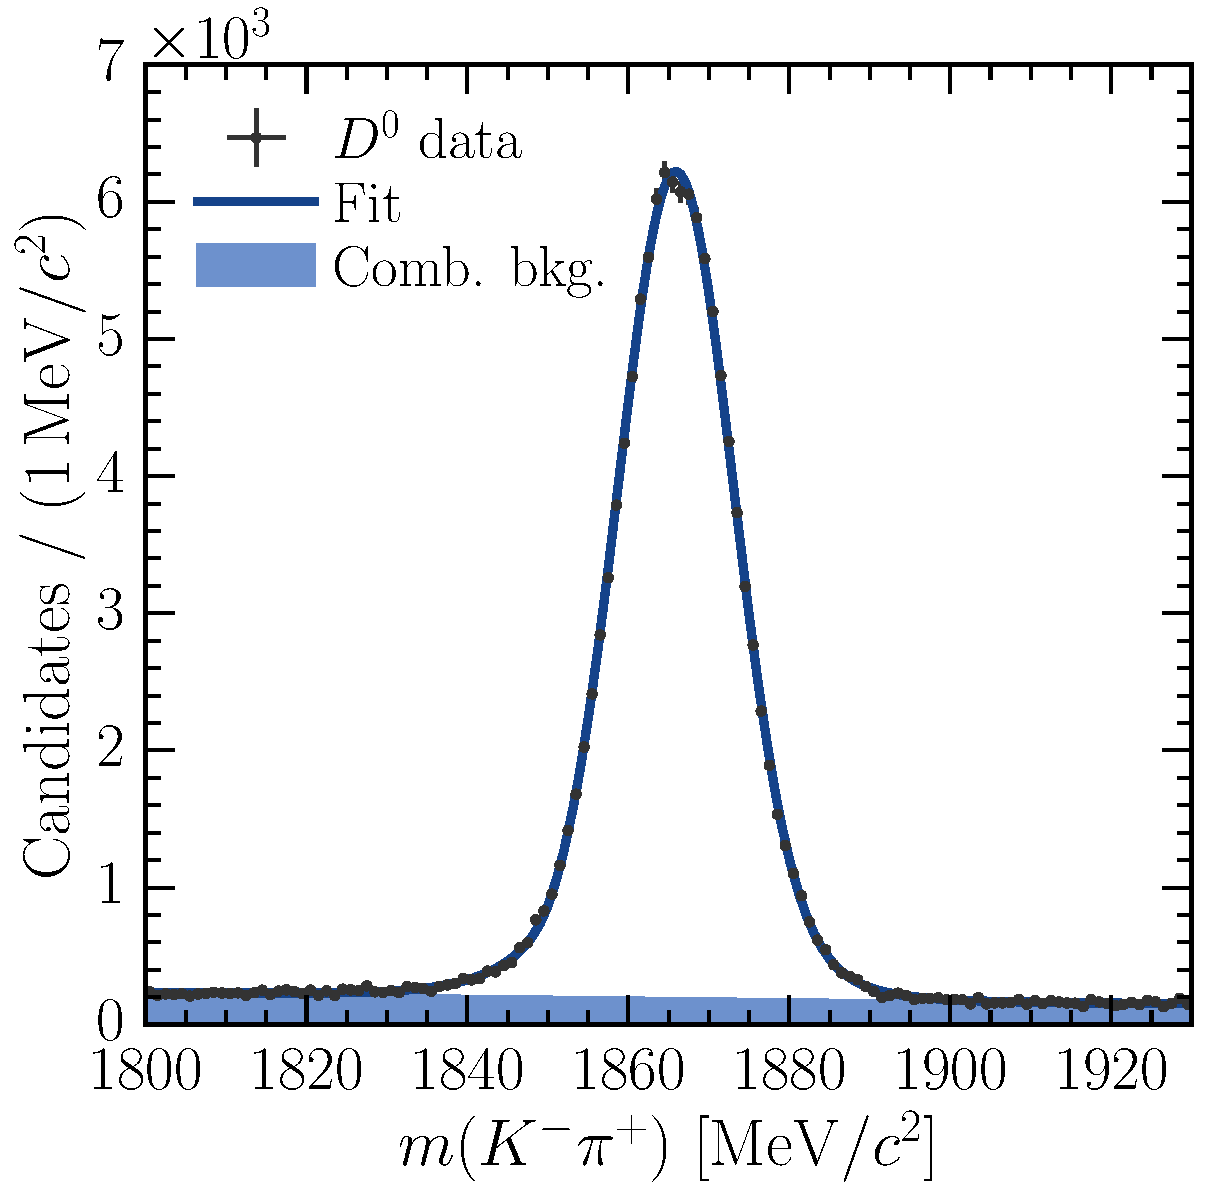
\includegraphics[width=\textwidth]{figures/production/fitting/D0ToKpi_mass_fit_pT_3_y_2}
    \caption{Mass}
    \label{fig:prod:fitting:D0ToKpi:mass_high_sig}
  \end{subfigure}
  \begin{subfigure}[b]{0.5\textwidth}
    \centering
    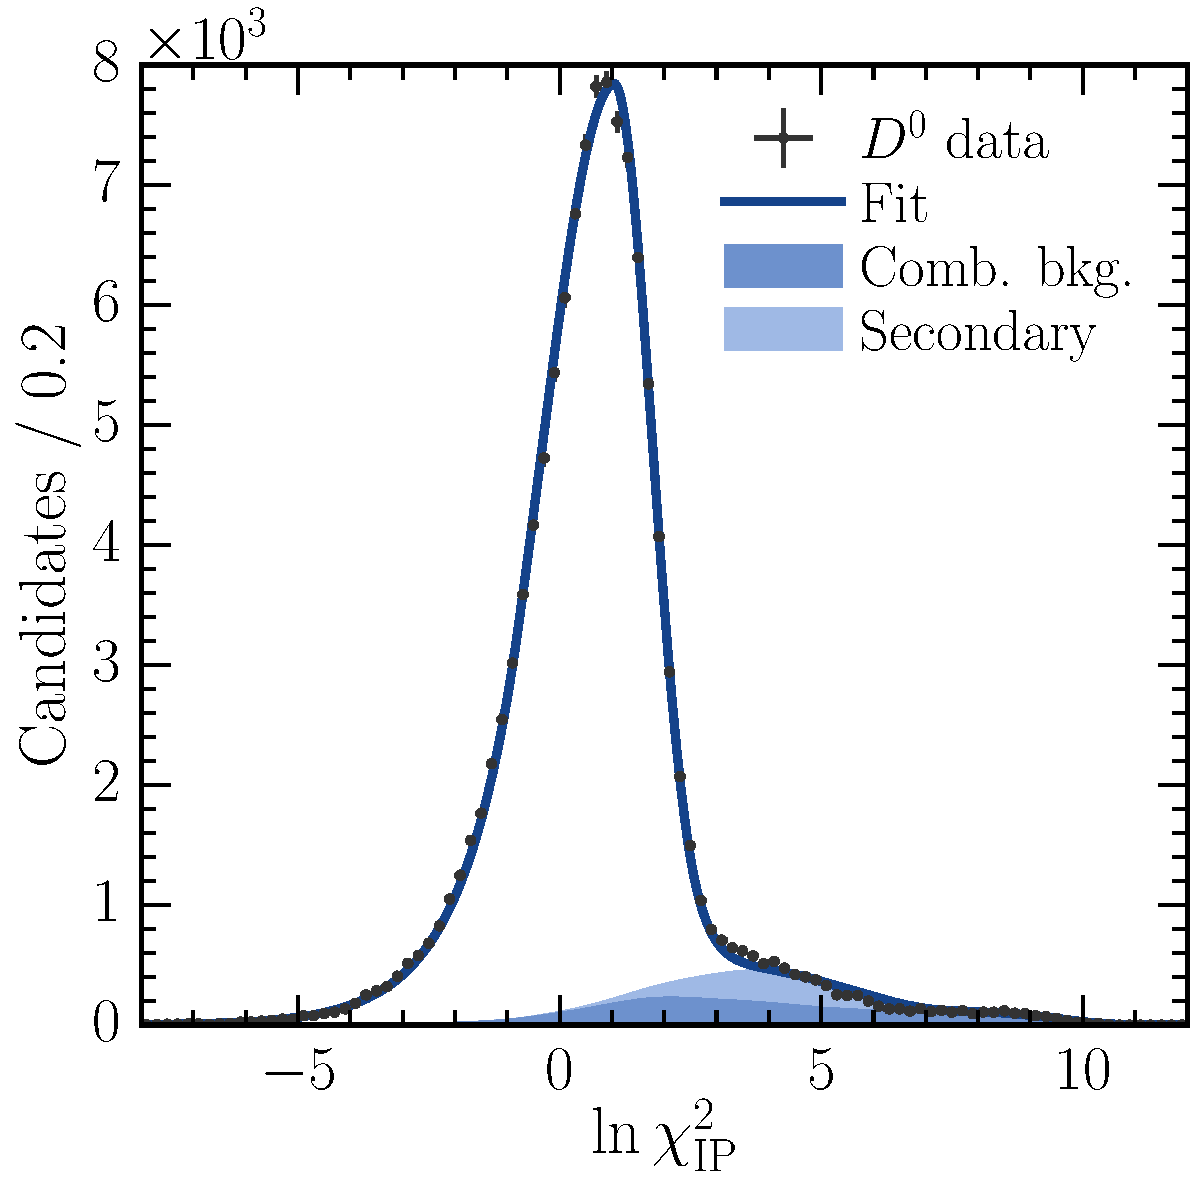
\includegraphics[width=\textwidth]{figures/production/fitting/D0ToKpi_ipchisq_fit_pT_3_y_2}
    \caption{\lnipchisq}
    \label{fig:prod:fitting:D0ToKpi:ipchisq_high_sig}
  \end{subfigure}
  \begin{subfigure}[b]{0.5\textwidth}
    \centering
    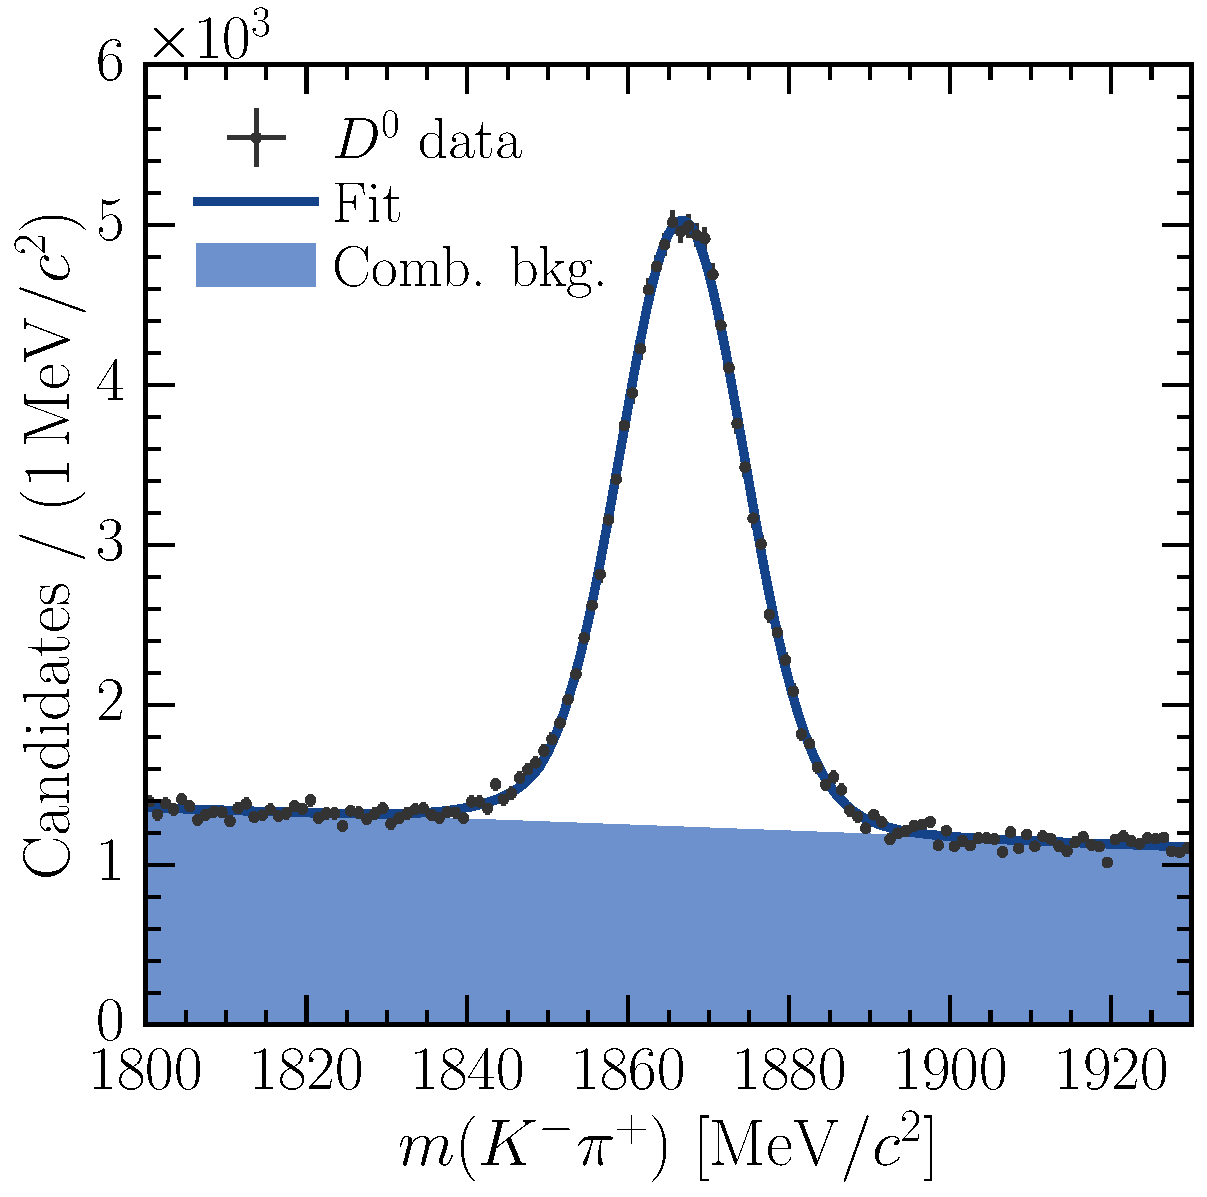
\includegraphics[width=\textwidth]{figures/production/fitting/D0ToKpi_mass_fit_pT_0_y_3}
    \caption{Mass}
    \label{fig:prod:fitting:D0ToKpi:mass_high_bkg}
  \end{subfigure}
  \begin{subfigure}[b]{0.5\textwidth}
    \centering
    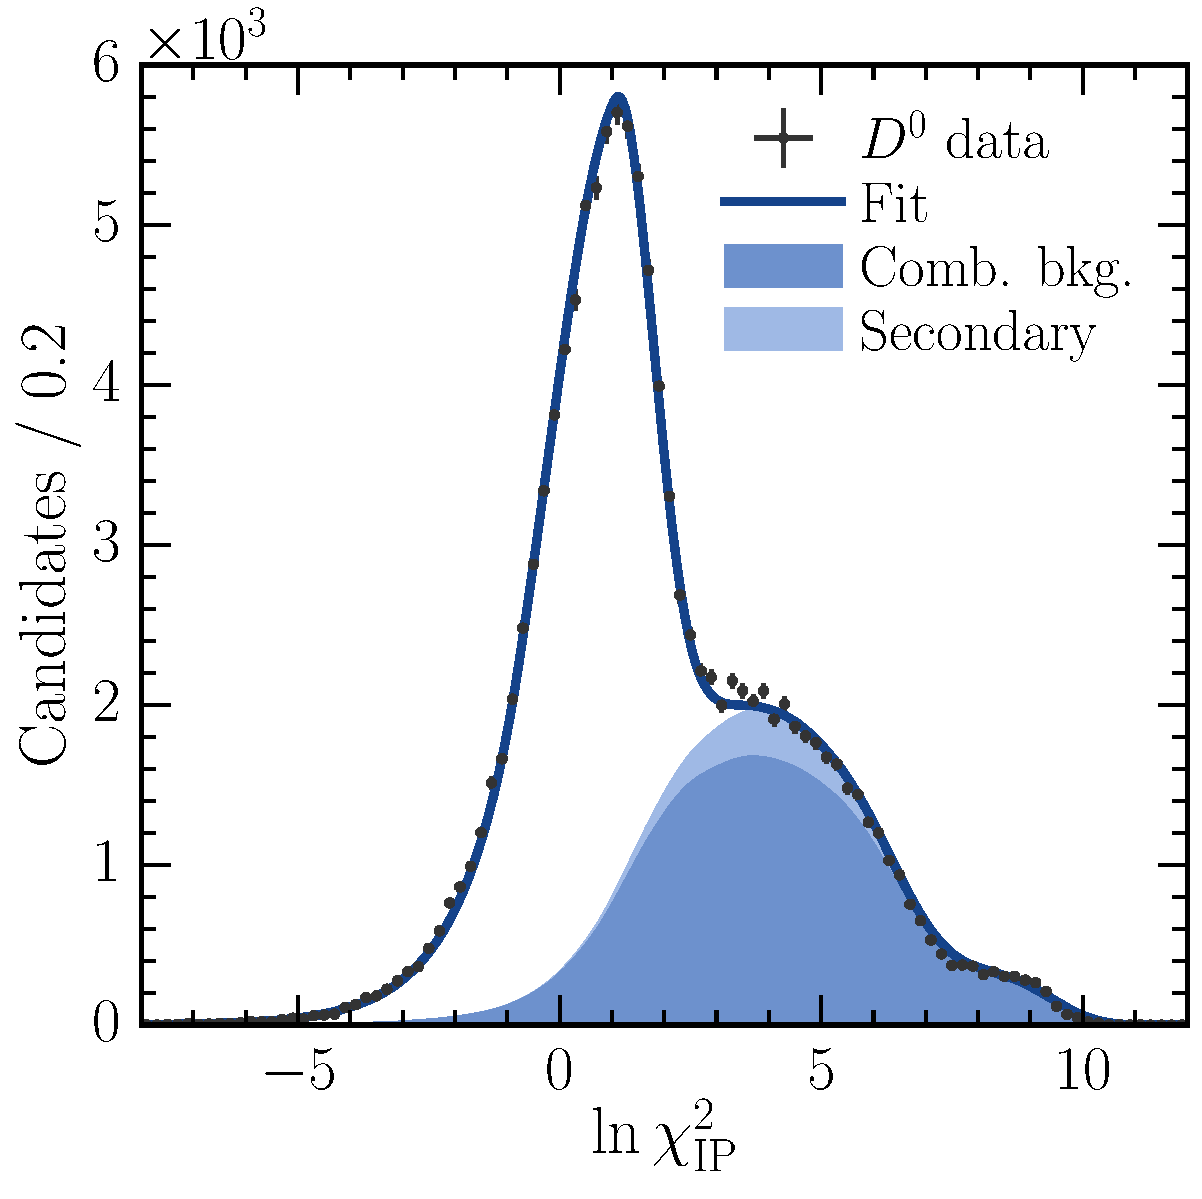
\includegraphics[width=\textwidth]{figures/production/fitting/D0ToKpi_ipchisq_fit_pT_0_y_3}
    \caption{\lnipchisq}
    \label{fig:prod:fitting:D0ToKpi:ipchisq_high_bkg}
  \end{subfigure}
  \caption{%
    Distributions for fully selected \DzToKpi\ candidates: \PDzero\ invariant 
    mass (\subref*{fig:prod:fitting:D0ToKpi:mass_high_sig} and 
    \subref*{fig:prod:fitting:D0ToKpi:mass_high_bkg}); and \PDzero\ \lnipchisq\ 
    (\subref*{fig:prod:fitting:D0ToKpi:ipchisq_high_sig} and 
    \subref*{fig:prod:fitting:D0ToKpi:ipchisq_high_bkg}) for a mass window of 
    $\pm\SI{20}{\MeV}$ around the nominal \PDzero mass.
    The top Figures (\subref*{fig:prod:fitting:D0ToKpi:mass_high_sig} and 
    \subref*{fig:prod:fitting:D0ToKpi:ipchisq_high_sig}) show the data and fits 
    in the region \pTyrange{2}{2.5}{3}{3.5}, whilst the bottom Figures 
    (\subref*{fig:prod:fitting:D0ToKpi:mass_high_bkg} and 
    \subref*{fig:prod:fitting:D0ToKpi:ipchisq_high_bkg}) show the data and fits 
    in the \pTyrange{0}{1}{3.5}{4} region.
  }
  \label{fig:prod:fitting:D0ToKpi:sig_bkg}
\end{figure}

\begin{figure}
  \begin{subfigure}[b]{0.5\textwidth}
    \centering
    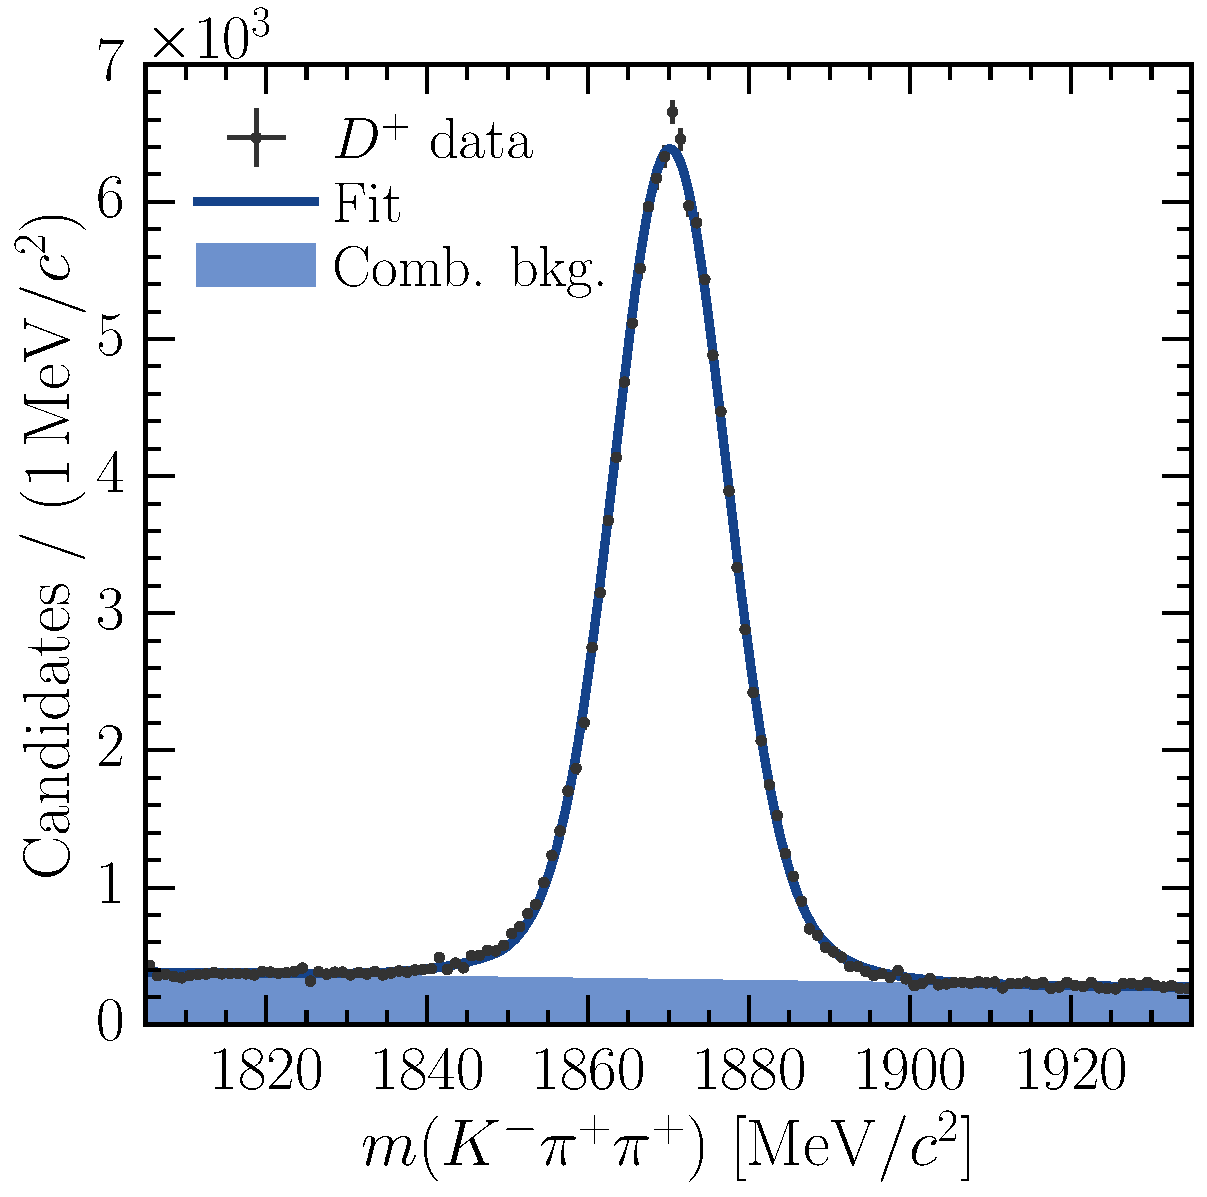
\includegraphics[width=\textwidth]{figures/production/fitting/DpToKpipi_mass_fit_pT_4_y_2}
    \caption{Mass}
    \label{fig:prod:fitting:DpToKpipi:mass_high_sig}
  \end{subfigure}
  \begin{subfigure}[b]{0.5\textwidth}
    \centering
    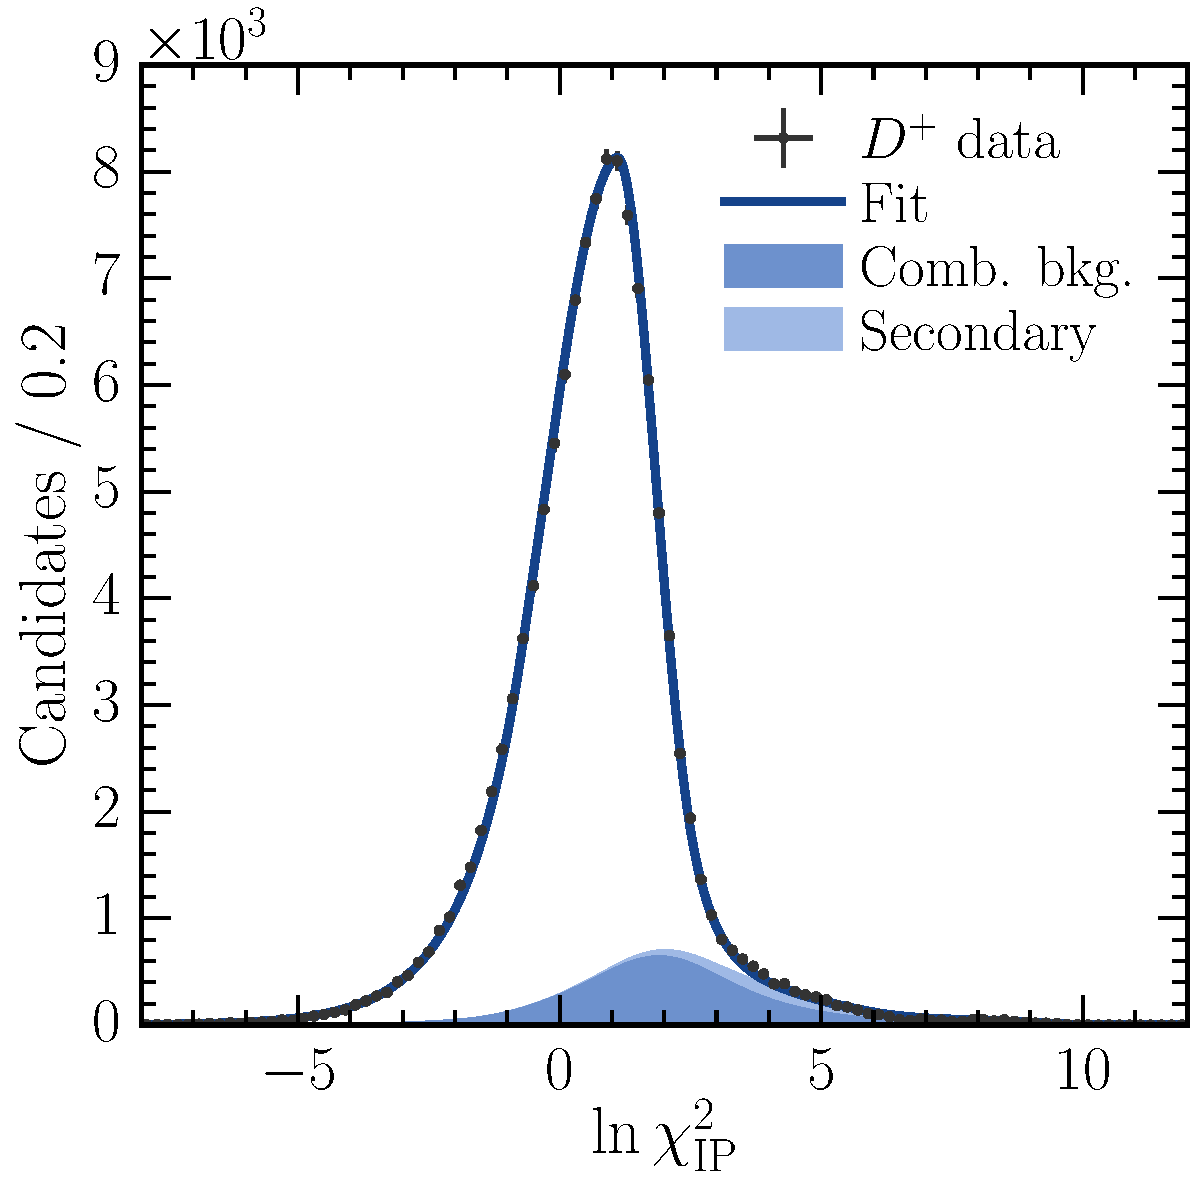
\includegraphics[width=\textwidth]{figures/production/fitting/DpToKpipi_ipchisq_fit_pT_4_y_2}
    \caption{\lnipchisq}
    \label{fig:prod:fitting:DpToKpipi:ipchisq_high_sig}
  \end{subfigure}
  \begin{subfigure}[b]{0.5\textwidth}
    \centering
    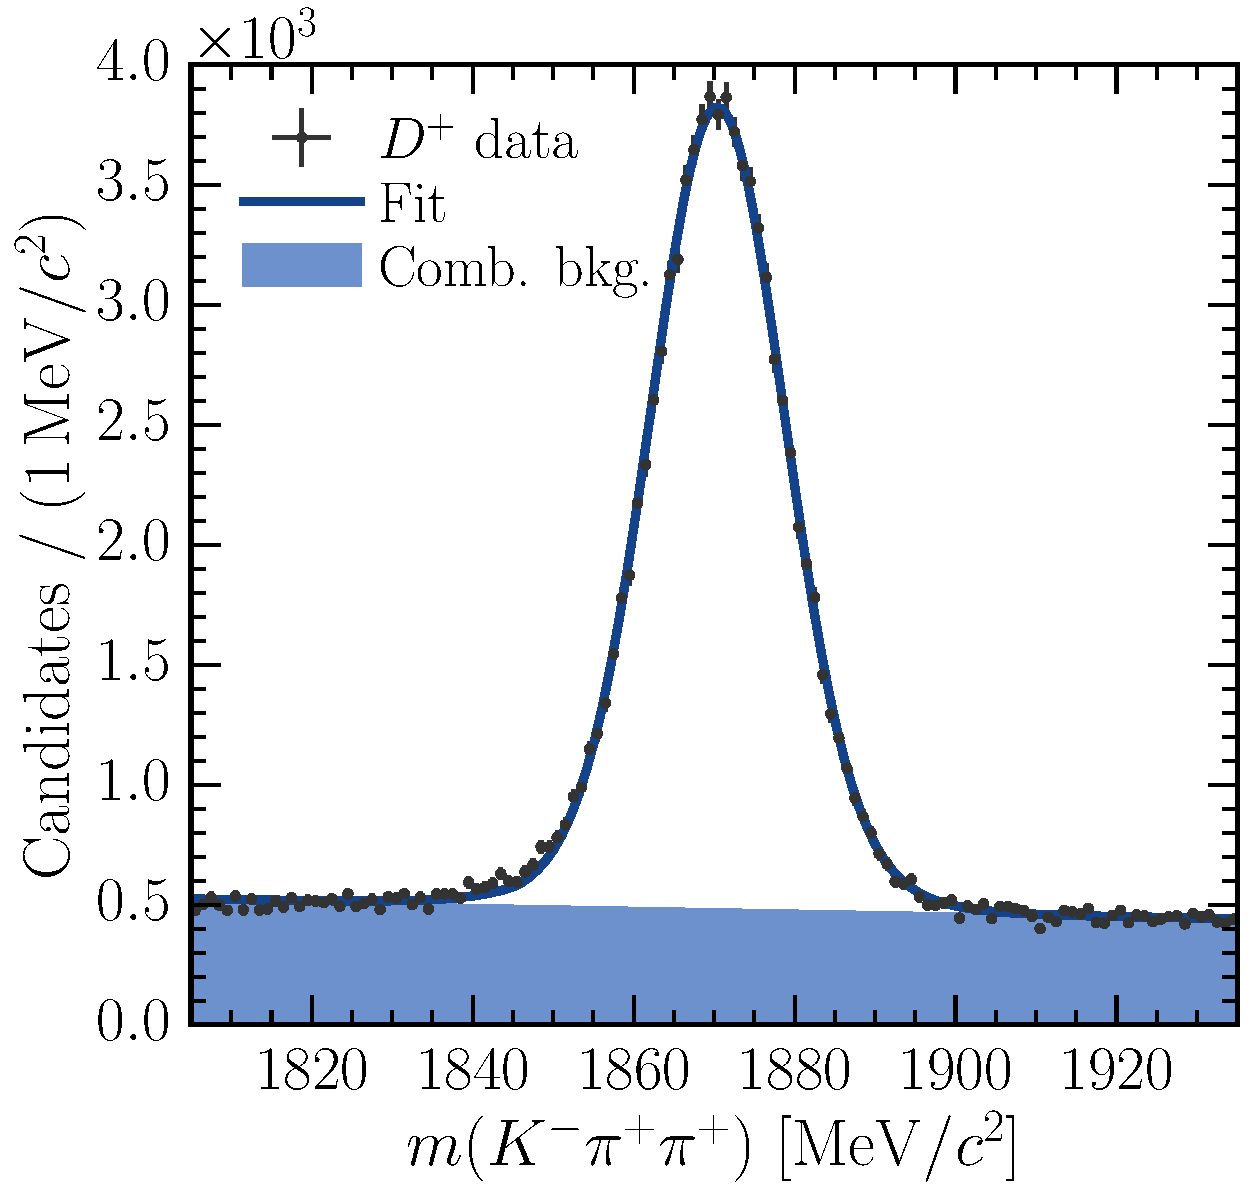
\includegraphics[width=\textwidth]{figures/production/fitting/DpToKpipi_mass_fit_pT_3_y_3}
    \caption{Mass}
    \label{fig:prod:fitting:DpToKpipi:mass_high_bkg}
  \end{subfigure}
  \begin{subfigure}[b]{0.5\textwidth}
    \centering
    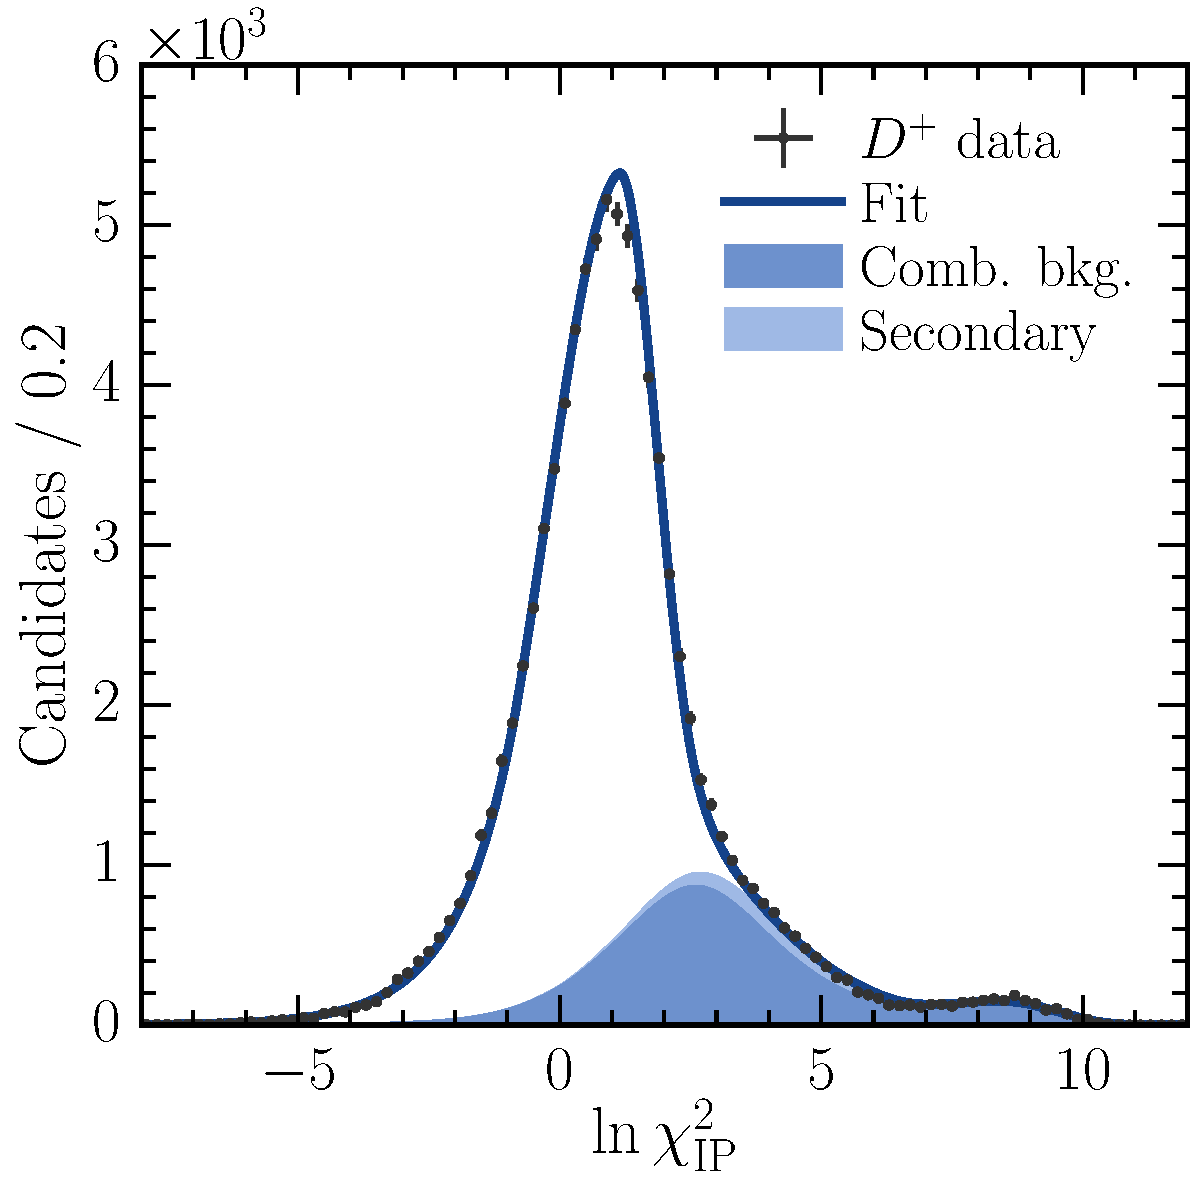
\includegraphics[width=\textwidth]{figures/production/fitting/DpToKpipi_ipchisq_fit_pT_3_y_3}
    \caption{\lnipchisq}
    \label{fig:prod:fitting:DpToKpipi:ipchisq_high_bkg}
  \end{subfigure}
  \caption{%
    Distributions for fully selected \DpToKpipi\ candidates: \PDplus\ invariant 
    mass (\subref*{fig:prod:fitting:DpToKpipi:mass_high_sig} and 
    \subref*{fig:prod:fitting:DpToKpipi:mass_high_bkg}); and \PDplus\ 
    \lnipchisq\ (\subref*{fig:prod:fitting:DpToKpipi:ipchisq_high_sig} and 
    \subref*{fig:prod:fitting:DpToKpipi:ipchisq_high_bkg}) for a mass window of 
    $\pm\SI{20}{\MeV}$ around the nominal \PDplus mass.
    The top Figures (\subref*{fig:prod:fitting:DpToKpipi:mass_high_sig} and 
    \subref*{fig:prod:fitting:DpToKpipi:ipchisq_high_sig}) show the data and 
    fits in the region \pTyrange{2.5}{3}{3}{3.5}, whilst the bottom Figures 
    (\subref*{fig:prod:fitting:DpToKpipi:mass_high_bkg} and 
    \subref*{fig:prod:fitting:DpToKpipi:ipchisq_high_bkg}) show the data and 
    fits in the \pTyrange{2}{2.5}{3.5}{4} region.
  }
  \label{fig:prod:fitting:DpToKpipi:sig_bkg}
\end{figure}

\begin{figure}
  \begin{subfigure}[b]{0.5\textwidth}
    \centering
    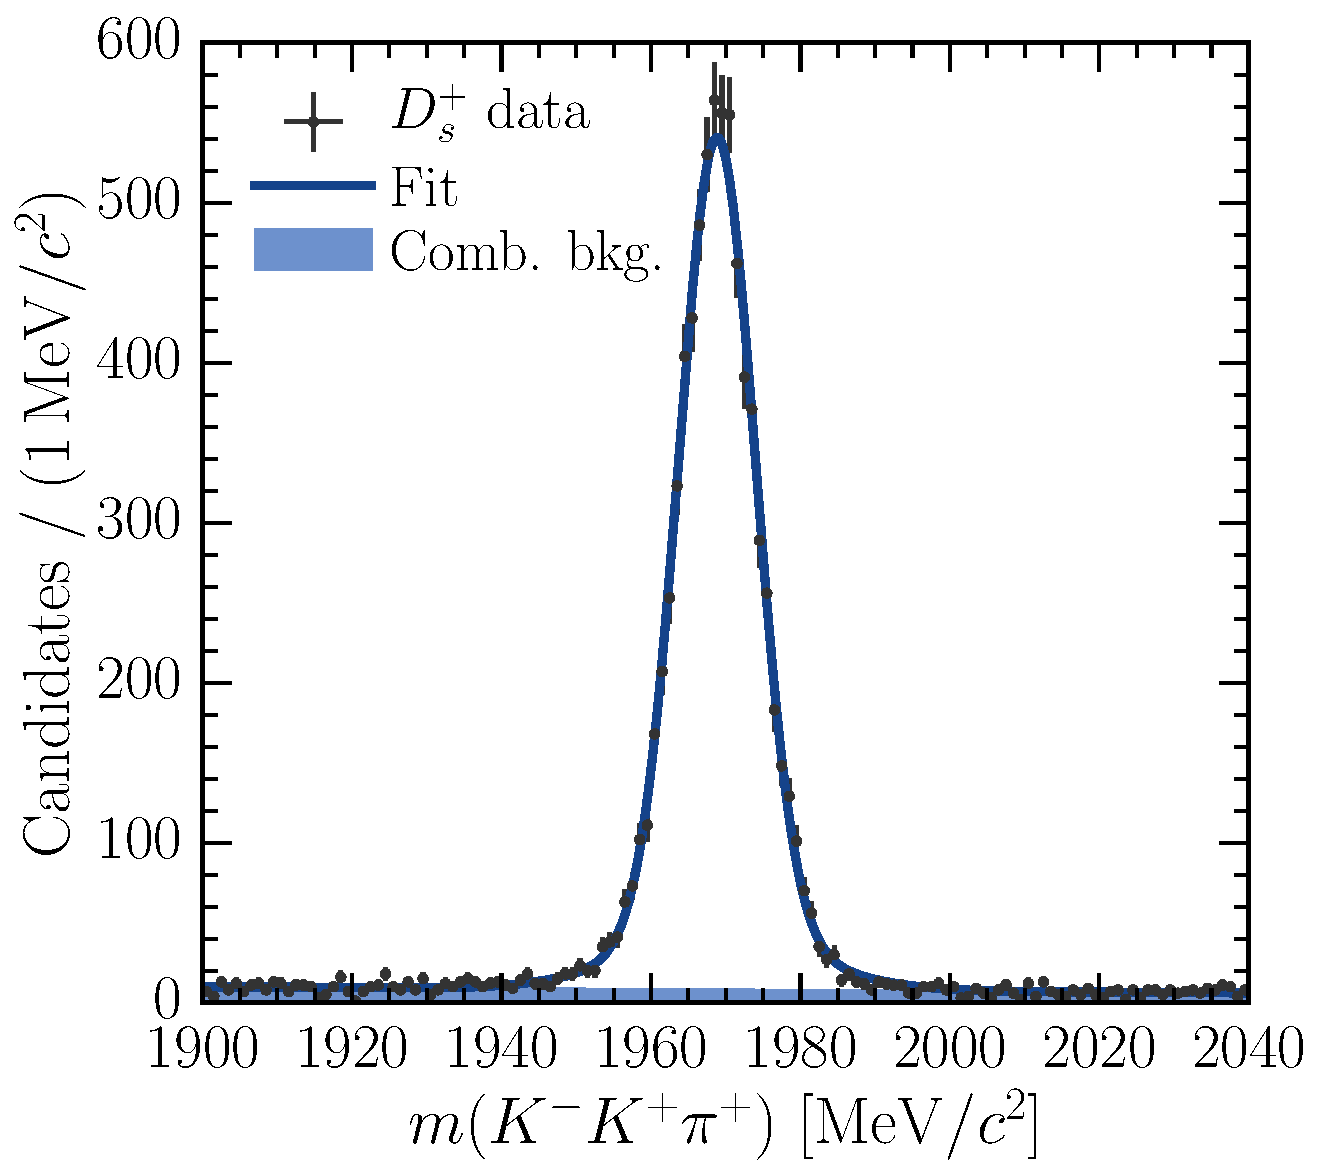
\includegraphics[width=\textwidth]{figures/production/fitting/DsToKKpi_mass_fit_pT_6_y_1}
    \caption{Mass}
    \label{fig:prod:fitting:DsToKKpi:mass_high_sig}
  \end{subfigure}
  \begin{subfigure}[b]{0.5\textwidth}
    \centering
    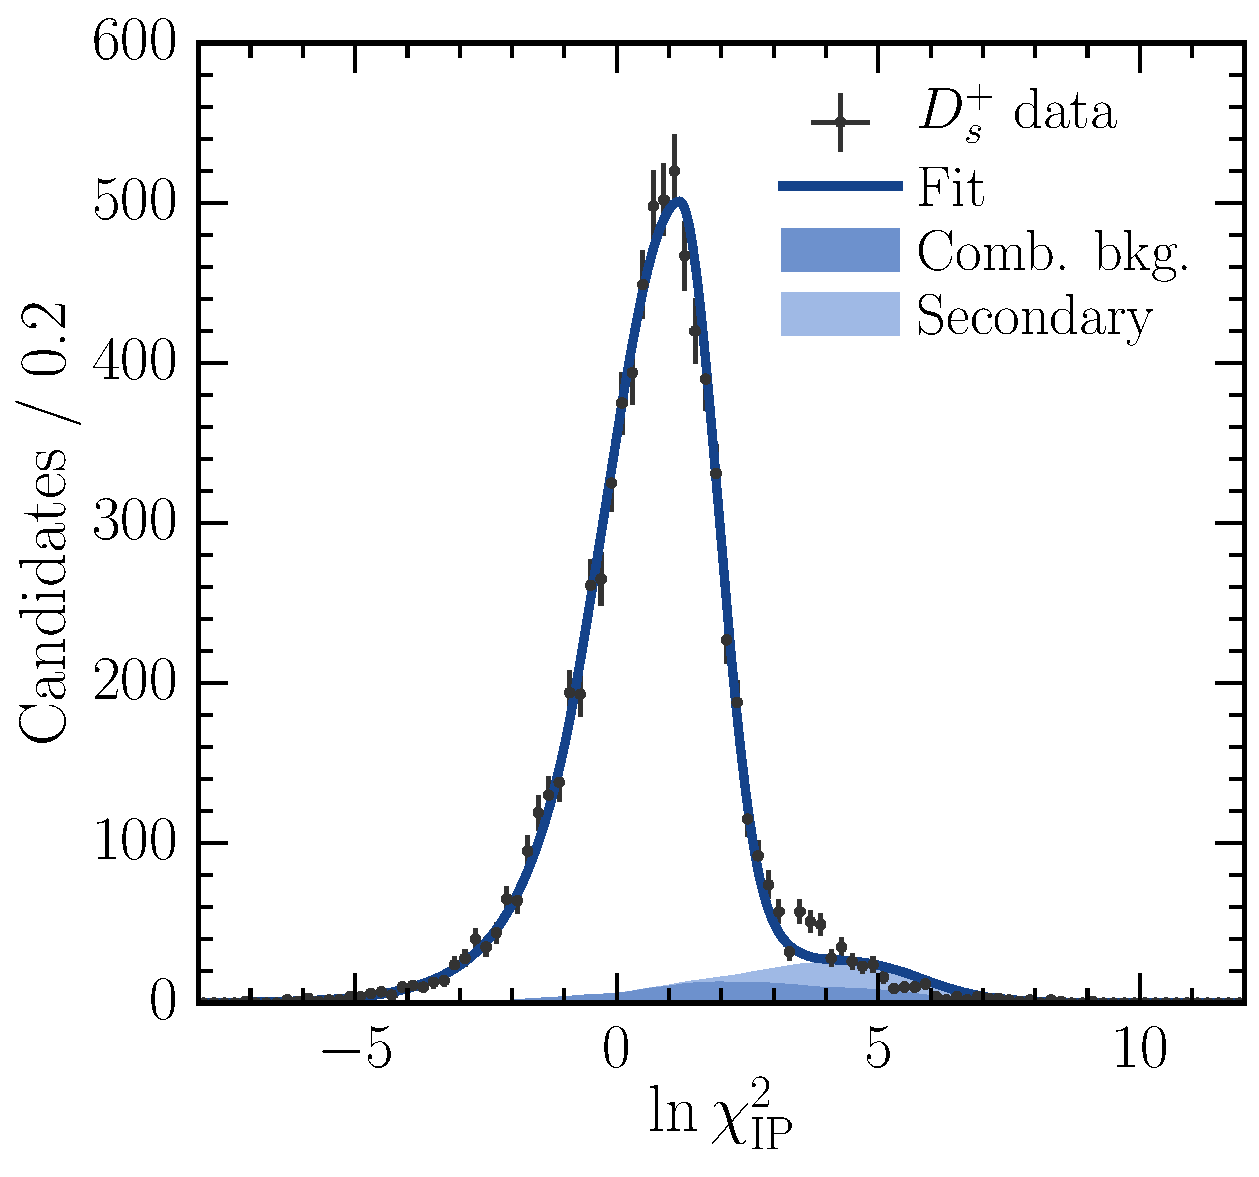
\includegraphics[width=\textwidth]{figures/production/fitting/DsToKKpi_ipchisq_fit_pT_6_y_1}
    \caption{\lnipchisq}
    \label{fig:prod:fitting:DsToKKpi:ipchisq_high_sig}
  \end{subfigure}
  \begin{subfigure}[b]{0.5\textwidth}
    \centering
    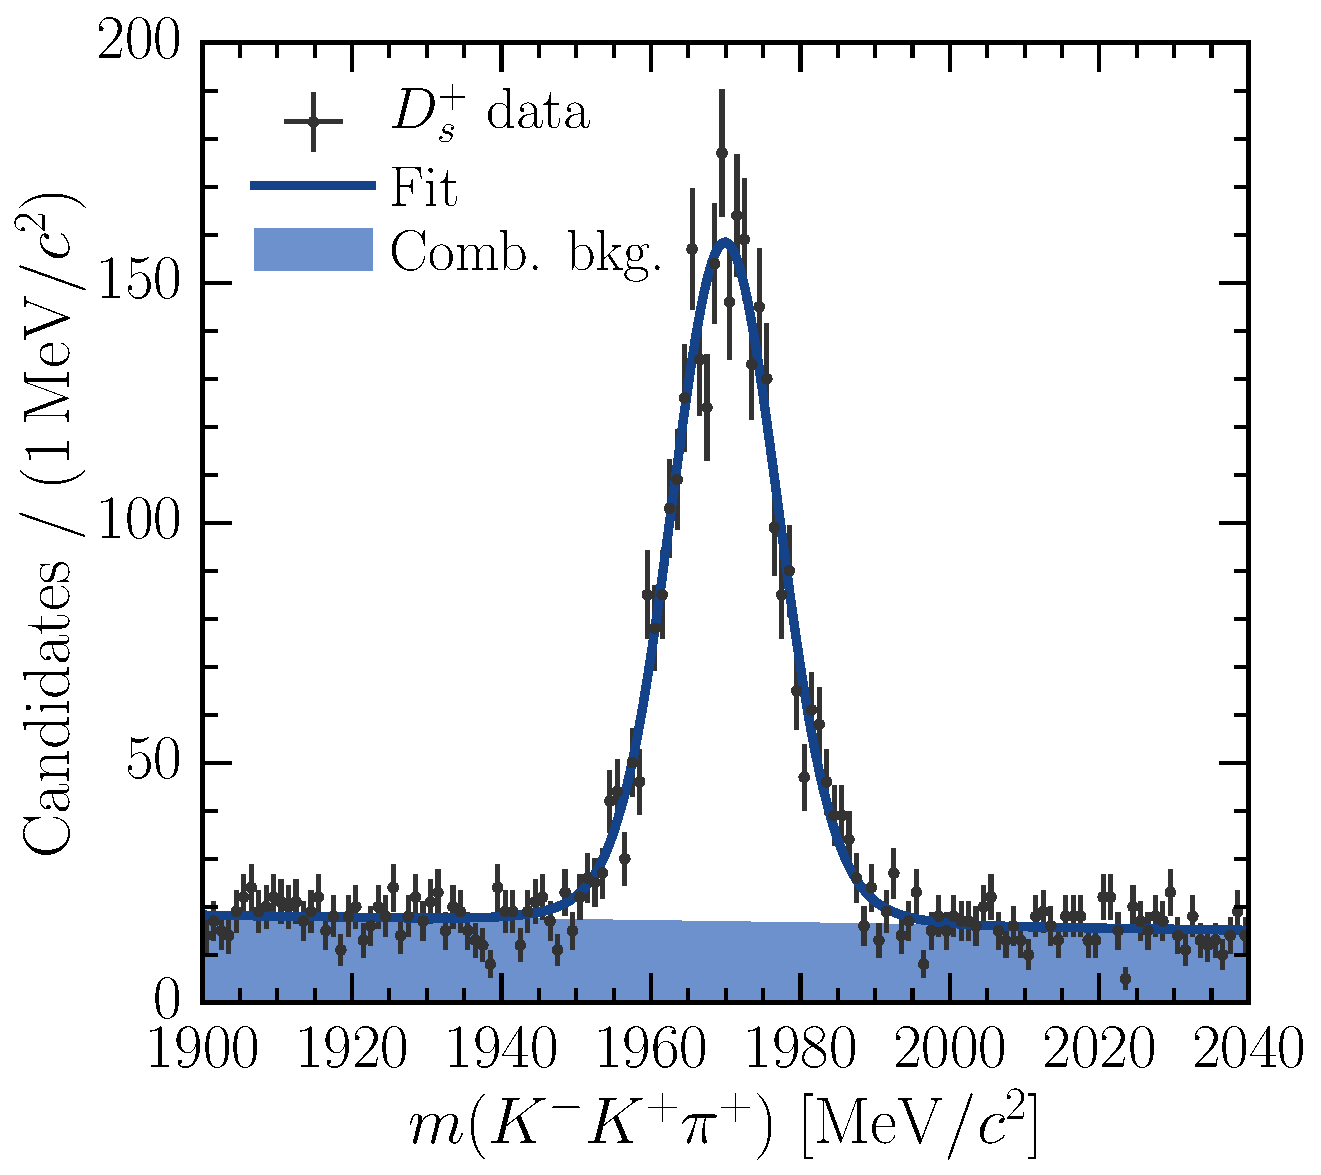
\includegraphics[width=\textwidth]{figures/production/fitting/DsToKKpi_mass_fit_pT_2_y_3}
    \caption{Mass}
    \label{fig:prod:fitting:DsToKKpi:mass_high_bkg}
  \end{subfigure}
  \begin{subfigure}[b]{0.5\textwidth}
    \centering
    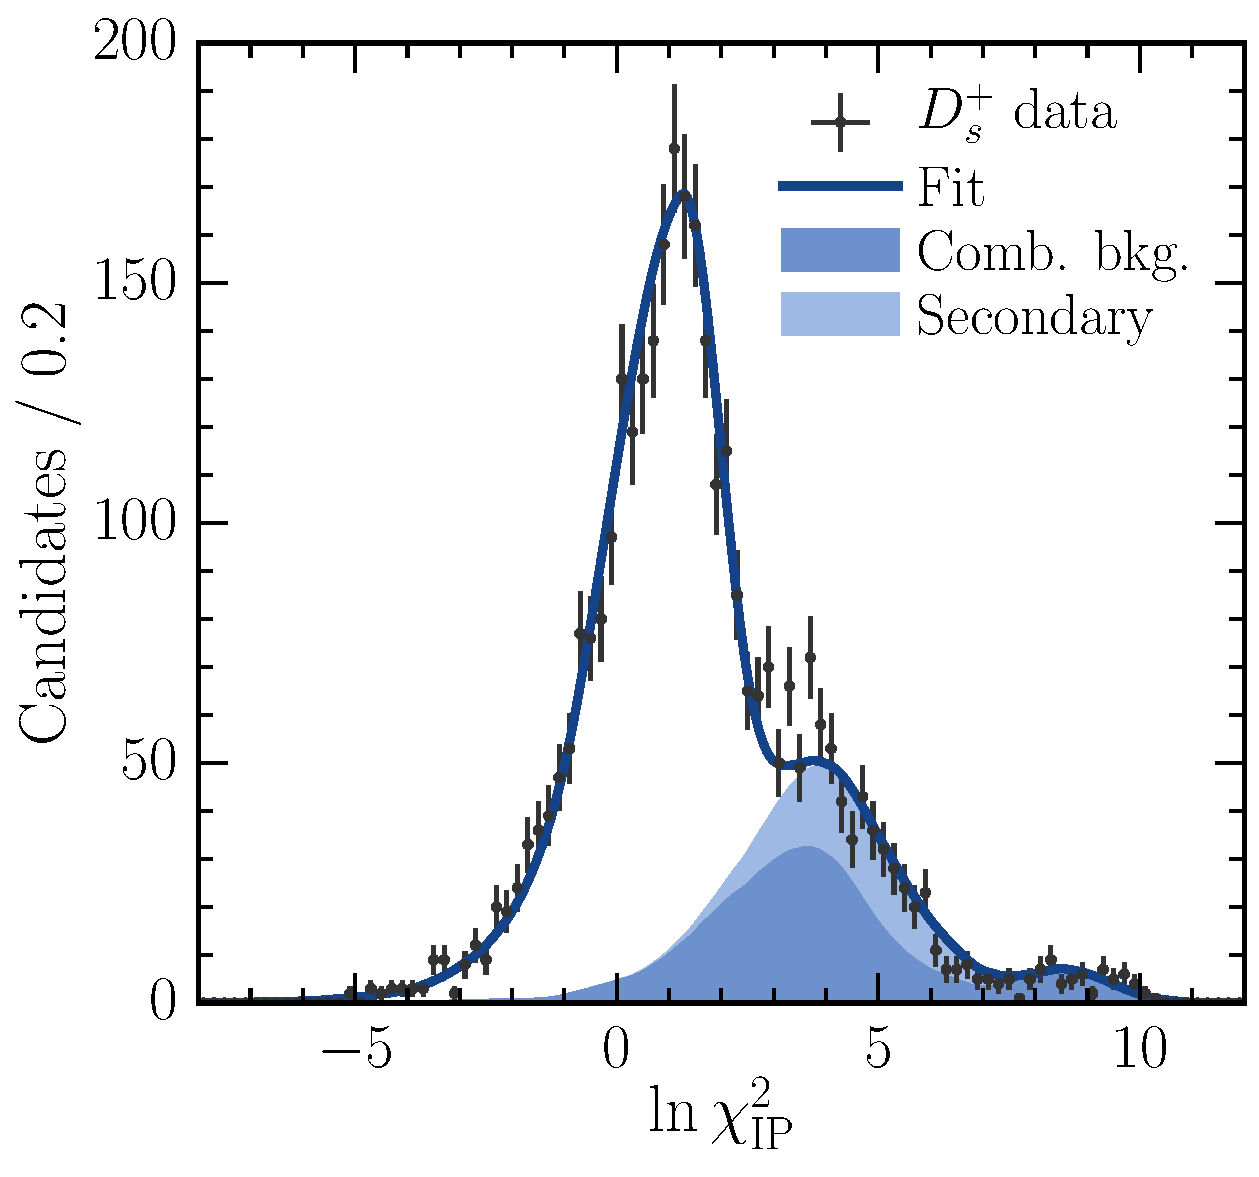
\includegraphics[width=\textwidth]{figures/production/fitting/DsToKKpi_ipchisq_fit_pT_2_y_3}
    \caption{\lnipchisq}
    \label{fig:prod:fitting:DsToKKpi:ipchisq_high_bkg}
  \end{subfigure}
  \caption{%
    Distributions for fully selected \DspTophipi\ candidates: \PDsplus\ 
    invariant mass (\subref*{fig:prod:fitting:DsToKKpi:mass_high_sig} and 
    \subref*{fig:prod:fitting:DsToKKpi:mass_high_bkg}); and \PDsplus\ 
    \lnipchisq\ (\subref*{fig:prod:fitting:DsToKKpi:ipchisq_high_sig} and 
    \subref*{fig:prod:fitting:DsToKKpi:ipchisq_high_bkg}) for a mass window of 
    $\pm\SI{20}{\MeV}$ around the nominal \PDsplus mass.
    The top Figures (\subref*{fig:prod:fitting:DsToKKpi:mass_high_sig} and 
    \subref*{fig:prod:fitting:DsToKKpi:ipchisq_high_sig}) show the data and 
    fits in the region \pTyrange{4}{5}{2.5}{3}, whilst the bottom Figures 
    (\subref*{fig:prod:fitting:DsToKKpi:mass_high_bkg} and 
    \subref*{fig:prod:fitting:DsToKKpi:ipchisq_high_bkg}) show the data and 
    fits in the \pTyrange{2}{2.5}{3.5}{4} region.
  }
  \label{fig:prod:fitting:DsToKKpi:sig_bkg}
\end{figure}

\begin{figure}
  \begin{subfigure}[b]{0.5\textwidth}
    \centering
    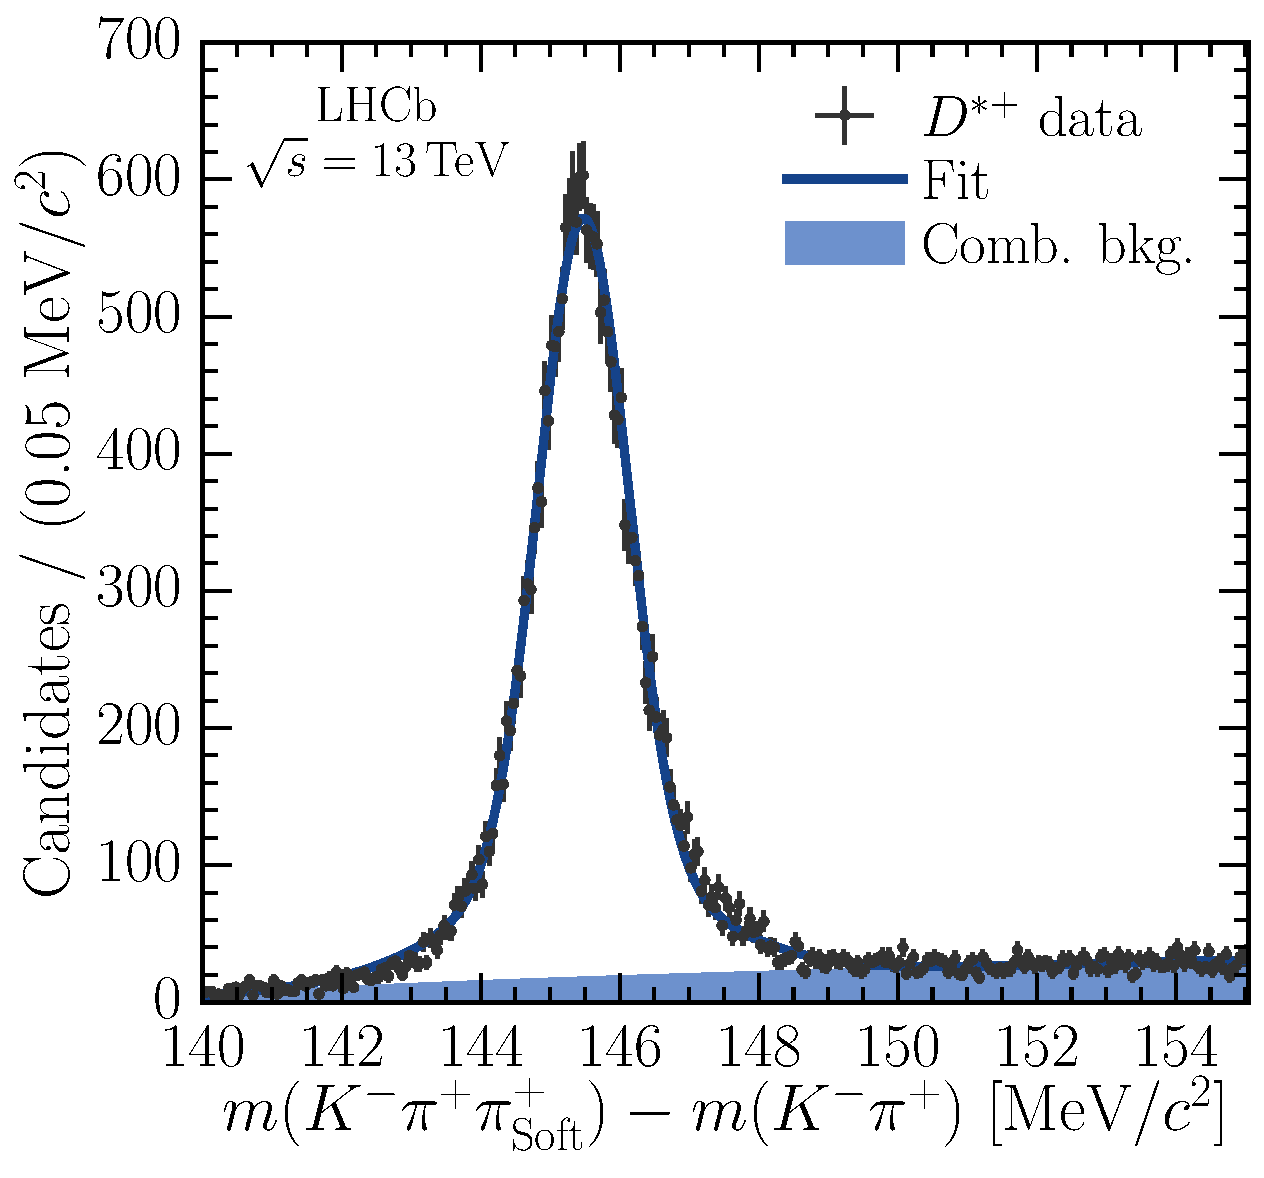
\includegraphics[width=\textwidth]{figures/production/fitting/DstToD0pi_D0ToKpi_delta_mass_fit_pT_7_y_2}
    \caption{Delta mass}
    \label{fig:prod:fitting:DstToD0pi_D0ToKpi:delta_mass_high_sig}
  \end{subfigure}
  \begin{subfigure}[b]{0.5\textwidth}
    \centering
    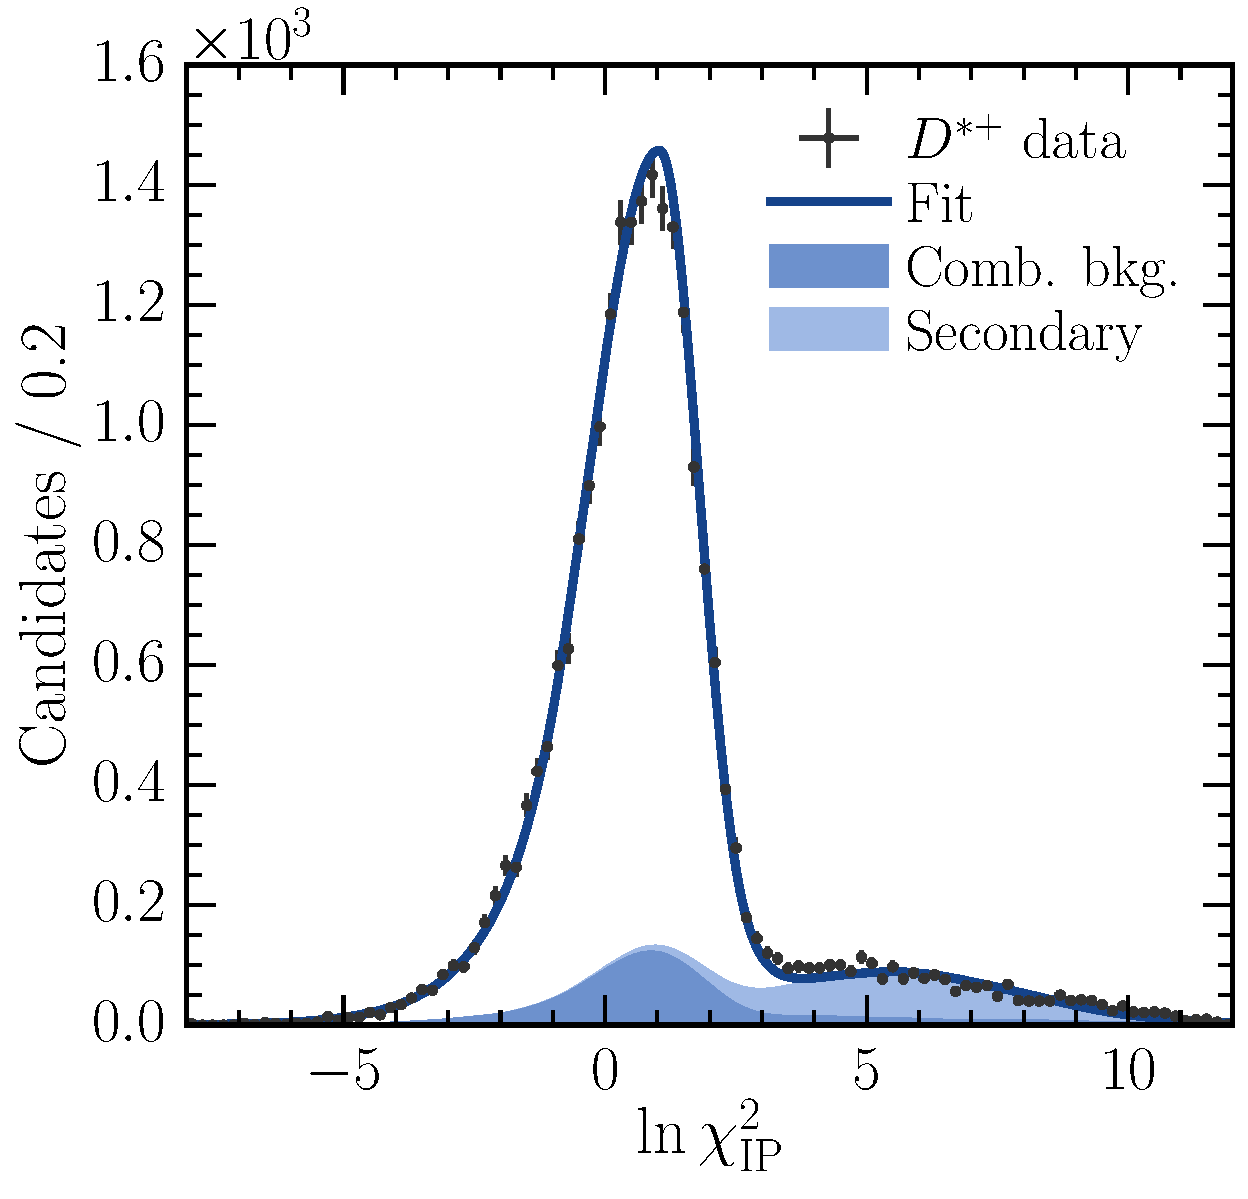
\includegraphics[width=\textwidth]{figures/production/fitting/DstToD0pi_D0ToKpi_ipchisq_fit_pT_7_y_2}
    \caption{\lnipchisq}
    \label{fig:prod:fitting:DstToD0pi_D0ToKpi:ipchisq_high_sig}
  \end{subfigure}
  \begin{subfigure}[b]{0.5\textwidth}
    \centering
    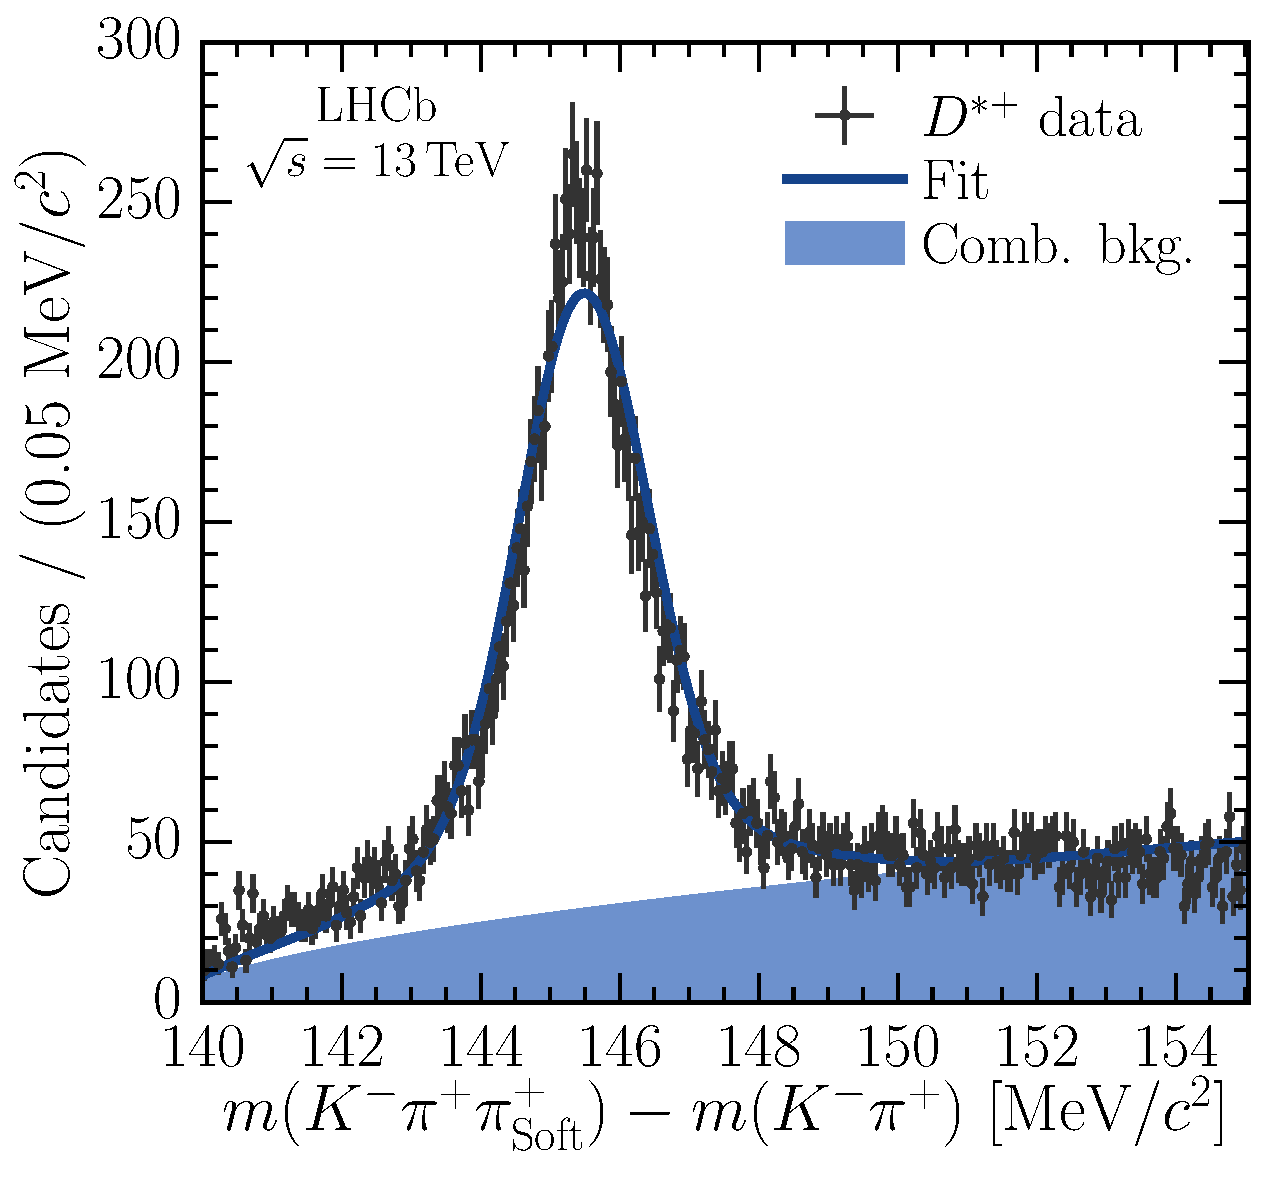
\includegraphics[width=\textwidth]{figures/production/fitting/DstToD0pi_D0ToKpi_delta_mass_fit_pT_2_y_3}
    \caption{Delta mass}
    \label{fig:prod:fitting:DstToD0pi_D0ToKpi:delta_mass_high_bkg}
  \end{subfigure}
  \begin{subfigure}[b]{0.5\textwidth}
    \centering
    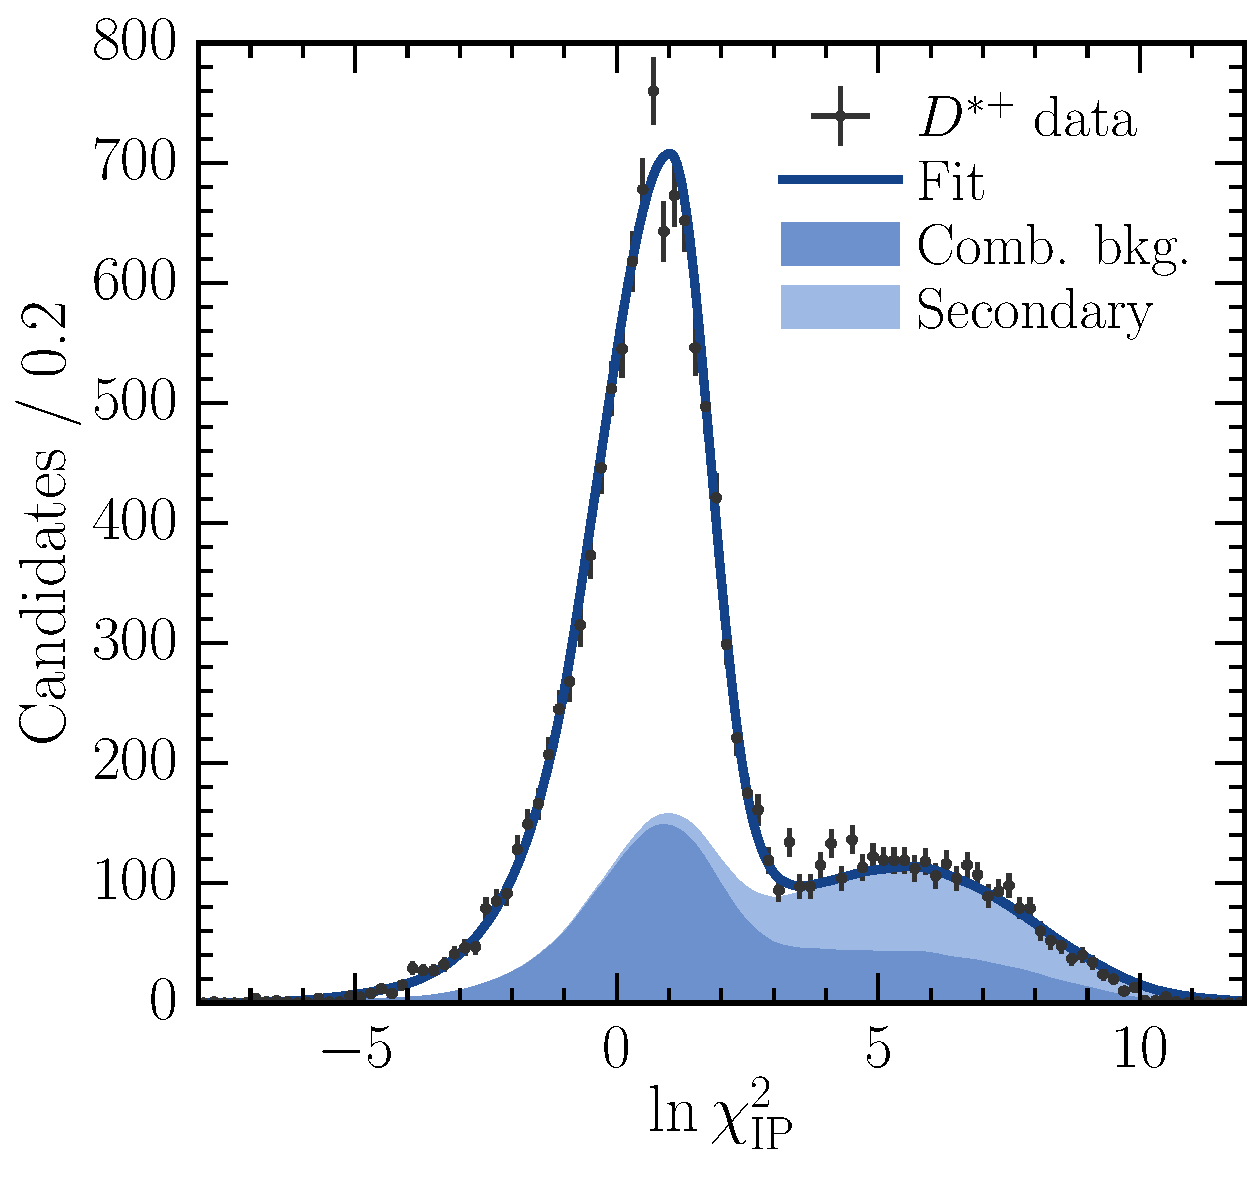
\includegraphics[width=\textwidth]{figures/production/fitting/DstToD0pi_D0ToKpi_ipchisq_fit_pT_2_y_3}
    \caption{\lnipchisq}
    \label{fig:prod:fitting:DstToD0pi_D0ToKpi:ipchisq_high_bkg}
  \end{subfigure}
  \caption{%
    Distributions for fully selected \DstToDzpi, with \DzToKpi, candidates: 
    $\deltam = m(\PDstarp) - m(\PDzero)$ 
    (\subref*{fig:prod:fitting:DstToD0pi_D0ToKpi:delta_mass_high_sig} and 
    \subref*{fig:prod:fitting:DstToD0pi_D0ToKpi:delta_mass_high_bkg}) for a 
    mass window of $\pm\SI{20}{\MeV}$ around the nominal \PDzero mass; and 
    \PDzero\ \lnipchisq\ 
    (\subref*{fig:prod:fitting:DstToD0pi_D0ToKpi:ipchisq_high_sig} and 
    \subref*{fig:prod:fitting:DstToD0pi_D0ToKpi:ipchisq_high_bkg}) with an 
    additional mass window of $\pm\SI{3}{\MeV}$ around the nominal 
    \PDstarp-\PDzero\ mass difference.
    The top Figures 
    (\subref*{fig:prod:fitting:DstToD0pi_D0ToKpi:delta_mass_high_sig} and 
    \subref*{fig:prod:fitting:DstToD0pi_D0ToKpi:ipchisq_high_sig}) show the 
    data and fits in the region \pTyrange{4}{5}{3}{3.5}, whilst the bottom 
    Figures (\subref*{fig:prod:fitting:DstToD0pi_D0ToKpi:delta_mass_high_bkg} 
    and \subref*{fig:prod:fitting:DstToD0pi_D0ToKpi:ipchisq_high_bkg}) show the 
    data and fits in the \pTyrange{1.5}{2}{3.5}{4} region.
  }
  \label{fig:prod:fitting:DstToD0pi_D0ToKpi:sig_bkg}
\end{figure}
